\chapter{Verificación y validación}
\label{CapituloPruebas}
\par En este capítulo se exponen los diferentes ciclos de verificación y validación llevados adelante durante el desarrollo de este proyecto. Según \cite{Press10} ``... La verificación se refiere al conjunto de tareas que garantizan que el software implementa correctamente una función específica. La validación es un conjunto diferente de tareas que aseguran que el software que se construye sigue los requerimientos del cliente.''.

% ACÁ DECIR Q VAMOS A TENER PRUEBAS DE INTEGRACIÓN, VALIDACIÓN Y SISTEMAS
% Integracion: Escenarios + Casos de Prueba
% Pruebas validación: Prueba Estática
%                     Prueba de Entrega: Escenarios + Casos de prueba.
% Pruebas de sistema: Rendimiento + Campo

\section{Plan de pruebas}
\par Los ciclos de verificación y validación de este sistema se plasman en los distintos tipos de pruebas realizadas sobre el sistema. A continuación se presenta el plan de pruebas para el sistema desarrollado. Dentro del cual, se señala y define cada tipo de prueba a ser llevada a cabo. 

\begin{itemize}
    \item{\textbf{Prueba de integración:}} El objetivo de este tipo de prueba es descubrir defectos en el sistema. El proceso de integración del sistema implica construir éste a partir de sus componentes, y probar el sistema resultante con el fin de descubrir conflictos que pudiesen surgir producto de la interacción entre ellos. Este tipo de prueba también es conocido como prueba de caja blanca, ya que se tiene acceso al código fuente. Las mismas son realizadas por el equipo de desarrollo.
    
    \item{\textbf{Prueba de validación:}} El objetivo de estas pruebas es demostrar la conformidad con los requerimientos definidos para el sistema construido. Las pruebas para este fin son indicadas a continuación. 
    
        \begin{itemize}
            \item{\textbf{Prueba estática de validación de requerimientos:}} Su objetivo es asegurar el cumplimiento de todos los requerimientos definidos para el sistema. Se presenta una tabla en la cual se chequean los requerimientos funcionales y no funcionales en contraposición al sistema desarrollado.
            \item{\textbf{Pruebas de entrega:}} También conocidas como “pruebas funcionales” o “pruebas de caja negra”, plasmadas en casos de prueba donde el único interés es el de validar las funcionalidades del sistema, sin considerar su implementación.
        \end{itemize}
        
    \item{\textbf{Prueba del sistema:}} Según \cite{Press10} ``La prueba del sistema verifica que todos los elementos se mezclan de manera adecuada y que se logra el funcionamiento/rendimiento global del sistema''. Luego son indicadas las pruebas realizadas con este objetivo.
        \begin{itemize}
            \item{\textbf{Pruebas de rendimiento:}} El fin de este tipo de pruebas es validar que el sistema cumple los requerimientos de rendimiento. Se basa en mediciones sobre el sistema para determinar que éste ofrezca las funcionalidades dentro de los límites establecidos para cada característica evaluada.
            \item{\textbf{Pruebas de campo:}} Se somete el sistema construido a condiciones de operación reales y se verifica que el mismo funcione de la forma esperada.
        \end{itemize}
\end{itemize}

\section{ Pruebas de integración }
\par En esta sección se detallan los escenarios y, posteriormente, los casos de prueba utilizados para llevar a cabo las pruebas de integración.


\subsection{Escenarios}
\par Se presentan ejemplos de escenarios a ser considerados para la creación o generación de casos de pruebas. 
% Escenarios => CP

% Prueba de valores actuales => Sensor desconectado, api no trae datos.

% Planificación de maceración => Intentar poner datos que corresponden o dejar vacíos, típica rotura de formulario.

% Inicio moni? ... no se me ocurre nada para romper.

% Monitorización de maceración en curso => Interrupción de funcionamiento / Desconexión, Cerrar la app en el transcurso de la medición

%Finalización de moni? Se olvidó de poner la densidad

%En la evaluación de maceración no se me ocurre nada por ahora para romper, porque la base de datos esta en el teléfono.


%ESCENARIO 1  
\begin{longtable}{|p{2cm}|p{12cm}|}
    \hline
    \multicolumn{2}{|c|}{ Escenario 01 : Informar valores actuales } \\
    \hline
    \hline
    \endfirsthead
    
    \hline
    \caption{Escenario 01}\\
    \endfoot
    
    \hline
    \multicolumn{2}{|c|}{Continuación de la Tabla \ref{tab:TablaEscenario01}}\\
    \hline
    \hline
    \endhead
    
    \hline
    \caption{Escenario 01 \label{tab:TablaEscenario01}}\\
    \endlastfoot


    %%%%%% tbody %%%%%%%%
    Objetivo
    & Visualizar valores obtenidos por todos los sensores \\
    \hline
    
    Contexto
    & El usuario tiene montado el sistema de recolección de datos, el sistema conectado a la red inalámbrica y la aplicación abierta en la pantalla principal.
    \\
    \hline
    
    Recursos
    &
    \begin{itemize}
        \item Sistema de recolección de datos.
        \item Aplicación móvil.
    \end{itemize}
    \\
    \hline
    
    Actor
    & Productor de cerveza
    \\
    \hline
    
    Episodios
    & \begin{itemize}
        \item El usuario selecciona el botón flotante ubicado en la pantalla principal.
        \item La aplicación muestra un dialogo pop-up con un \textit{spinner} de carga mientras espera la respuesta de la API.
        \item La aplicación enseña los valores obtenidos por cada uno de los sensores de la estación obtenidos recientemente.
    \end{itemize}
    \\
    \hline
    
    Caso alternativo
    & \begin{itemize}
        \item La aplicación no recibe respuesta de la API y enseña el mensaje ``Error de conexión con el servidor''.
    \end{itemize}
    \\
    \hline
    %%% end tbody
\end{longtable}

  %ESCENARIO 02 

\begin{longtable}{|p{2cm}|p{12cm}|}
    \hline
    \multicolumn{2}{|c|}{ Escenario 02 : Nueva Maceración } \\
    \hline
    \hline
    \endfirsthead
    
    \hline
    \caption{Escenario 02}\\
    \endfoot
    
    \hline
    \multicolumn{2}{|c|}{Continuación de la Tabla \ref{tab:TablaEscenario02}}\\
    \hline
    \hline
    \endhead
 
     \hline
    \caption{Escenario 02 \label{tab:TablaEscenario02}}\\
    \endlastfoot


    %%%%%% tbody %%%%%%%%
    Objetivo
    & Dar de alta un nueva receta de Maceración    \\
    \hline
    
    Contexto
    & El usuario abre la aplicación móvil.
    \\
    \hline
    
    Recursos
    & 
    \begin{itemize}
        \item Dispositivo móvil.
        \item Aplicación.
    \end{itemize} 
    \\
    \hline
    
    Actor
    & Productor de cerveza
    \\
    \hline
    
    Episodios
    & \begin{itemize}
        \item El usuario abre la aplicación en su dispositivo móvil.
        \item El usuario hace click en el botón ``+'' para agregar una nueva receta de maceración.
        \item El usuario ingresa la información necesaria para dar de alta una nueva maceración.
        \item El sistema crea la nueva receta.
        \item El sistema agrega la nueva receta a lista de recetas.
    \end{itemize}
    \\
    \hline
    
    Caso alternativo
    & \begin{itemize}
        \item El sistema no crea la nueva receta e informa la causa.
    \end{itemize}
    \\
    \hline

 \end{longtable}

%ESCENARIO 03
\begin{longtable}{|p{2cm}|p{12cm}|}
    \hline
    \multicolumn{2}{|c|}{ Escenario 03 : Realizar experimento} \\
    \hline
    \hline
    \endfirsthead
    
    \hline
    \caption{Escenario 03}\\
    \endfoot
    
    \hline
    \multicolumn{2}{|c|}{Continuación de la Tabla \ref{tab:TablaEscenario03}}\\
    \hline
    \hline
    \endhead
    
    \hline
    \caption{Escenario 03 \label{tab:TablaEscenario03}}\\
    \endlastfoot


    %%%%%% tbody %%%%%%%%
    Objetivo
    & Monitorear un experimento de maceración \\
    \hline
    
    Contexto
    & El usuario tiene montado el sistema de recolección de datos, el sistema conectado a la red inalámbrica y la aplicación abierta en la pantalla de gestión de maceración.
    \\
    \hline
    
    Recursos
    &
    \begin{itemize}
        \item Sistema de recolección de datos.
        \item Aplicación móvil.
    \end{itemize} 
    \\
    \hline
    
    Actor
    & Productor de cerveza
    \\
    \hline
    
    Episodios
    & \begin{itemize}
        \item El usuario selecciona el botón flotante ubicado en la pantalla de gestión de maceración.
        \item La aplicación muestra en la pantalla de monitoreo de experimento con los datos del experimento en curso.
        \item La aplicación indica que el experimento finalizó y muestra un dialogo para que se inserte la densidad obtenida.
        \item El usuario inserta el valor de densidad.
    \end{itemize}
    \\
    \hline
    
    Caso alternativo
    & \begin{itemize}
        \item La aplicación no recibe respuesta de la API y cancela el experimento superado cierto lapso de tiempo definido.
        \item La aplicación detecta un desvío respecto a la planificación y enseña una notificación.
    \end{itemize}
    \\
    \hline
    %%% end tbody
\end{longtable}

  %ESCENARIO 04 

\begin{longtable}{|p{2cm}|p{12cm}|}
    \hline
    \multicolumn{2}{|c|}{ Escenario 04 : Eliminar maceración } \\
    \hline
    \hline
    \endfirsthead
    
    \hline
    \caption{Escenario 04}\\
    \endfoot
    
    \hline
    \multicolumn{2}{|c|}{Continuación de la Tabla \ref{tab:TablaEscenario04}}\\
    \hline
    \hline
    \endhead
 
     \hline
    \caption{Escenario 04 \label{tab:TablaEscenario04}}\\
    \endlastfoot


    %%%%%% tbody %%%%%%%%
    Objetivo
    & Eliminar una receta de Maceración    \\
    \hline
    
    Contexto
    & El usuario abre la aplicación móvil.
    \\
    \hline
    
    Recursos
    & 
    \begin{itemize}
        \item Dispositivo móvil.
        \item Aplicación.
    \end{itemize} 
    \\
    \hline
    
    Actor
    & Productor de cerveza
    \\
    \hline
    
    Episodios
    & \begin{itemize}
        \item El usuario hace click en una receta de maceración.
        \item El sistema despliega el panel de gestión de maceración.
        \item El usuario hace click en el botón para eliminar la receta de maceración.
        \item El sistema valida la acción con el usuario.
        \item El sistema elimina la receta de maceración de la base de datos, y remueve la misma de la lista de recetas.
    \end{itemize}
    \\
    \hline
    
    Caso alternativo
    & \begin{itemize}
        \item El sistema no elimina la receta e informa la causa.
    \end{itemize}
    \\
    \hline

 \end{longtable}

  %ESCENARIO 05

\begin{longtable}{|p{2cm}|p{12cm}|}
    \hline
    \multicolumn{2}{|c|}{ Escenario 05 : Acceso a los datos históricos y estadísticos de una receta} \\
    \hline
    \hline
    \endfirsthead
    
    \hline
    \caption{Escenario 05}\\
    \endfoot
    
    \hline
    \multicolumn{2}{|c|}{Continuación de la Tabla \ref{tab:TablaEscenario05}}\\
    \hline
    \hline
    \endhead
 
     \hline
    \caption{Escenario 05 \label{tab:TablaEscenario05}}\\
    \endlastfoot


    %%%%%% tbody %%%%%%%%
    Objetivo
    & Acceder al panel panel de datos históricos y estadísticos de una receta de maceración   \\
    \hline
    
    Contexto
    & El usuario abre la aplicación móvil.
    \\
    \hline
    
    Recursos
    & 
    \begin{itemize}
        \item Dispositivo móvil.
        \item Aplicación.
    \end{itemize} 
    \\
    \hline
    
    Actor
    & Productor de cerveza
    \\
    \hline
    
    Episodios
    & \begin{itemize}
        \item El usuario hace click en una receta de maceración.
        \item El sistema despliega el panel de gestión de maceración.
        \item El usuario hace click en el botón para acceder al panel de datos históricos y estadísticos.
        \item El sistema despliega el panel de datos históricos y estadísticos.
    \end{itemize}
    \\
    \hline
    
    Caso alternativo
    &    \\
    \hline

 \end{longtable}

%%%% ESCENARIO 6 %%%%%
\begin{longtable}{|p{2cm}|p{12cm}|}
    \hline
    \multicolumn{2}{|c|}{ Escenario 06 : Eliminar experimento } \\
    \hline
    \hline
    \endfirsthead
    
    \hline
    \caption{Escenario 06}\\
    \endfoot
    
    \hline
    \multicolumn{2}{|c|}{Continuación de la Tabla \ref{tab:TablaEscenario06}}\\
    \hline
    \hline
    \endhead
 
     \hline
    \caption{Escenario 06 \label{tab:TablaEscenario06}}\\
    \endlastfoot


    %%%%%% tbody %%%%%%%%
    Objetivo
    & Eliminar una receta de maceración    \\
    \hline
    
    Contexto
    & El usuario abre la aplicación móvil.
    \\
    \hline
    
    Recursos
    & 
    \begin{itemize}
        \item Dispositivo móvil.
        \item Aplicación.
    \end{itemize} 
    \\
    \hline
    
    Actor
    & Productor de cerveza
    \\
    \hline
    
    Episodios
    & \begin{itemize}
        \item El usuario hace click en una receta de maceración.
        \item El sistema despliega el panel de gestión de maceración.
        \item El usuario mantiene seleccionado el ítem correspondiente al experimento que desea eliminar.
        \item El sistema valida la acción con el usuario.
        \item El sistema elimina el experimento de la base de datos, y remueve la misma de la lista de experimentos.
    \end{itemize}
    \\
    \hline
    
    Caso alternativo
    & \begin{itemize}
        \item El sistema no elimina el experimento e informa la causa.
    \end{itemize}
    \\
    \hline

 \end{longtable}
 
 
 %%%% ESCENARIO 7 %%%%%
\begin{longtable}{|p{2cm}|p{12cm}|}
    \hline
    \multicolumn{2}{|c|}{ Escenario 07 : Ver detalle de un experimento } \\
    \hline
    \hline
    \endfirsthead
    
    \hline
    \caption{Escenario 07}\\
    \endfoot
    
    \hline
    \multicolumn{2}{|c|}{Continuación de la Tabla \ref{tab:TablaEscenario07}}\\
    \hline
    \hline
    \endhead
 
     \hline
    \caption{Escenario 07 \label{tab:TablaEscenario07}}\\
    \endlastfoot


    %%%%%% tbody %%%%%%%%
    Objetivo
    & Eliminar una receta de maceración    \\
    \hline
    
    Contexto
    & El usuario abre la aplicación móvil.
    \\
    \hline
    
    Recursos
    & 
    \begin{itemize}
        \item Dispositivo móvil.
        \item Aplicación.
    \end{itemize} 
    \\
    \hline
    
    Actor
    & Productor de cerveza
    \\
    \hline
    
    Episodios
    & \begin{itemize}
        \item El usuario hace click en una receta de maceración.
        \item El sistema despliega el panel de gestión de maceración.
        \item El usuario selecciona un experimento de maceración.
        \item El sistema despliega una pantalla con el detalle del experimento de maceración llevado a cabo.
    \end{itemize}
    \\
    \hline
    
    Caso alternativo
    & \begin{itemize}
        \item El sistema no elimina el experimento e informa la causa.
    \end{itemize}
    \\
    \hline

 \end{longtable}

%%%%%% ESCENARIO 8 %%%%%%%
\begin{longtable}{|p{2cm}|p{12cm}|}
    \hline
    \multicolumn{2}{|c|}{ Escenario 08 : Acceso a detalle de maceración} \\
    \hline
    \hline
    \endfirsthead
    
    \hline
    \caption{Escenario 08}\\
    \endfoot
    
    \hline
    \multicolumn{2}{|c|}{Continuación de la Tabla \ref{tab:TablaEscenario08}}\\
    \hline
    \hline
    \endhead
 
     \hline
    \caption{Escenario 08 \label{tab:TablaEscenario08}}\\
    \endlastfoot


    %%%%%% tbody %%%%%%%%
    Objetivo
    & Acceder al panel panel de detalle de maceración   \\
    \hline
    
    Contexto
    & El usuario abre la aplicación móvil.
    \\
    \hline
    
    Recursos
    & 
    \begin{itemize}
        \item Dispositivo móvil.
        \item Aplicación.
    \end{itemize} 
    \\
    \hline
    
    Actor
    & Productor de cerveza
    \\
    \hline
    
    Episodios
    & \begin{itemize}
        \item El usuario hace click en una receta de maceración.
        \item El sistema despliega el panel de gestión de maceración.
        \item El usuario hace click en el botón para acceder al panel de detalle de maceración.
        \item El sistema despliega el detalle de maceración.
    \end{itemize}
    \\
    \hline
    
    Caso alternativo
    &    \\
    \hline

 \end{longtable}

\subsection{Casos de prueba}
A continuación se listan los casos de pruebas, siendo en cada caso indicado: nombre, tipo de prueba, descripción, objetivos, datos de entrada, salida esperada y salida obtenida.
%----------------- FICHA CASO DE PRUEBA 1------------------------

\begin{longtable}{|p{0.6cm}|p{4cm}|p{4.7cm}|p{4.7cm}|}
    \hline
    \multicolumn{4}{| p{0.95\linewidth} |}{\textbf{Caso de prueba  CP001: Verificar despliegue de mediciones en panel de valores actuales}}\\
    \hline
    \multicolumn{4}{| l |}{\textbf{Escenario:} 01 }\\
    \hline
    \multicolumn{4}{| l |}{\textbf{Tipo de prueba:} Prueba de integración}\\
    \hline
    \multicolumn{4}{| l |}{\textbf{Actor de caso de prueba:} Equipo de desarrollo}\\
    \hline
    \multicolumn{4}{| l |}{\textbf{Propósito}}\\
    \hline
    \multicolumn{4}{|p{0.95\linewidth}|}{Verificar la respuesta del panel del valores actuales ante la obtención de valores provenientes de sensores desconectados.}\\
    \hline
    \endfirsthead
 
    \hline
    \multicolumn{4}{|c|}{Continuación de la Tabla \ref{CasoDePrueba1}}\\
    \hline
    \endhead
 
    \hline
    \endfoot

    \hline 
    \caption{Ficha de caso de prueba CP001\label{CasoDePrueba1}}\\
    \endlastfoot
    
    \hline
    \multicolumn{4}{| l |}{\textbf{Objetivos}}\\
    \hline
    \multicolumn{4}{| p{0.95\linewidth} |}{
        \begin{itemize}
            \item Verificar que la aplicación indique la falta de conexión de los sensores desconectados.
            \item Verificar que el proceso de recolección de datos sea tolerante a fallos de algun/os de los sensor/es.
        \end{itemize}
    }\\
    \hline
    \multicolumn{4}{| l |}{\textbf{Descripción de acciones para las pruebas}}\\
    \hline
    \textbf{\#} & Datos de entrada & Salida esperada & Salida obtenida\\
    \hline
    01 & Se desconectan 2 sensores de temperatura y el de pH de la estación de recolección de datos.  &  &  \\
    \hline
    02 & Se abre el panel de valores actuales.  & La aplicación debería mostrar el panel de valores actuales, y para cada sensor desconectado, un valor fácilmente identificable como erróneo. & Se abre el panel de valores actuales, los sensores de temperatura 1 y 4 muestran el valor ``-10.000'', y el sensor de pH indica el valor ``-1''.  \\
    \hline
 \end{longtable}

%----------------- FICHA CASO DE PRUEBA 2------------------------
\begin{longtable}{|p{0.6cm}|p{4cm}|p{4.7cm}|p{4.7cm}|}
    \hline
    \multicolumn{4}{| p{0.95\linewidth} |}{\textbf{Caso de prueba CP002: Verificar validación de conexión en panel de valores actuales }}\\
    \hline
    \multicolumn{4}{| l |}{\textbf{Escenario:} 01 }\\
    \hline
    \multicolumn{4}{| l |}{\textbf{Tipo de prueba:} Prueba de integración}\\
    \hline
    \multicolumn{4}{| l |}{\textbf{Actor de caso de prueba:} Equipo de desarrollo}\\
    \hline
    \multicolumn{4}{| l |}{\textbf{Propósito}}\\
    \hline
    \multicolumn{4}{|p{0.95\linewidth}|}{Verificar el despliegue de un mensaje de error ante la eventual falta de respuesta de la estación de recolección de datos a consecuencia de la apertura del panel de valores actuales.}\\
    \hline
    \endfirsthead
 
    \hline
    \multicolumn{4}{|c|}{Continuación de la Tabla \ref{CasoDePrueba2}}\\
    \hline
    \endhead
 
    \hline
    \endfoot

    \hline 
    \caption{Ficha de caso de prueba CP002\label{CasoDePrueba2}}\\
    \endlastfoot
    
    \hline
    \multicolumn{4}{| l |}{\textbf{Objetivos}}\\
    \hline
    \multicolumn{4}{| p{0.95\linewidth} |}{
        \begin{itemize}
            \item Verificar que la aplicación no permanezca en un bucle infinito a la espera de respuestas de la estación de recolección de datos.
            \item Verificar que la aplicación informe al usuario de esta situación.
        \end{itemize}
    }\\
    \hline
    \multicolumn{4}{| l |}{\textbf{Descripción de acciones para las pruebas}}\\
    \hline
    \textbf{\#} & Datos de entrada & Salida esperada & Salida obtenida\\
    \hline
    01 & Se apaga la estación de recolección de datos o el punto de acceso WiFi  &  &  \\
    \hline
    02 & Se abre el panel de valores actuales en la aplicación móvil. & La aplicación debería mostrar un mensaje de error indicando que no pudo establecer la conexión. & Se abre el panel de valores actuales, el cual presenta un icono de carga hasta que se alcanza cierto límite de tiempo corto, luego, enseña el mensaje emergente "No se ha podido establecer una conexión con el servidor". \\
    \hline
 \end{longtable}


%----------------- FICHA CASO DE PRUEBA 3------------------------

\begin{longtable}{|p{0.6cm}|p{4cm}|p{4.7cm}|p{4.7cm}|}
    \hline
    \multicolumn{4}{| p{0.95\linewidth} |}{\textbf{Caso de prueba  CP003: Verificar la validación de campos requeridos para el alta de maceración}}\\
    \hline
    \multicolumn{4}{| l |}{\textbf{Escenario:} 02 }\\
    \hline
    \multicolumn{4}{| l |}{\textbf{Tipo de prueba:} Prueba de integración}\\
    \hline
    \multicolumn{4}{| l |}{\textbf{Actor de caso de prueba:} Equipo de desarrollo}\\
    \hline
    \multicolumn{4}{| l |}{\textbf{Propósito}}\\
    \hline
    \multicolumn{4}{|p{0.95\linewidth}|}{Verificar que la aplicación valide la completitud mínima de campos de ingreso de datos.}\\
    \hline
    \endfirsthead
 
    \hline
    \multicolumn{4}{|c|}{Continuación de la Tabla \ref{CasoDePrueba3}}\\
    \hline
    \endhead
 
    \hline
    \endfoot

    \hline 
    \caption{Ficha de caso de prueba CP003\label{CasoDePrueba3}}\\
    \endlastfoot
    
    \hline
    \multicolumn{4}{| l |}{\textbf{Objetivos}}\\
    \hline
    \multicolumn{4}{| p{0.95\linewidth} |}{
        \begin{itemize}
            \item Verificar que la aplicación proceda correctamente en el proceso de alta de una nueva receta.
            \item Verificar que la aplicación valide la carga de al menos una variedad de grano antes de dar de alta una receta de maceración. 
            \item Verificar que la aplicación valide la carga de al menos un intervalo de maceración antes de avanzar con el alta de la receta de maceración.
            \item Verificar que la aplicación requiera que se rellenen todos los campos para dar de alta una receta.
        \end{itemize}
    }\\
    \hline
    \multicolumn{4}{| l |}{\textbf{Descripción de acciones para las pruebas}}\\
    \hline
    \textbf{\#} & Datos de entrada & Salida esperada & Salida obtenida\\
    \hline
    01 & Se abre la aplicación y se realiza click sobre el signo ``+'' para agregar una nueva receta de maceración.  &  & Se abre en la aplicación móvil el formulario con los campos de ingreso para dar de alta una nueva maceración.  \\
    \hline
    02 & No se completa ningún campo y se hace click en el botón de confirmación para el alta de la receta de maceración. & El sistema debería alertar que no se han ingresado valores en los campos requeridos. & La aplicación despliega un mensaje indicando que no se han ingresado valores requeridos.  \\
    \hline
    03 & Se completa un campo, luego de lo cual se hace click en el botón de confirmación para el alta de la receta de maceración. Luego de esto, se completa otro campo y se presiona la confirmación. Se prosigue hasta ingresar todos los campos si el sistema lo permite. & En cada caso la aplicación debería informar que los campos requeridos no se completaron.  & El sistema emite, en cada caso, una alerta informando que los campos requeridos no fueron completados, y no se puede continuar con el alta de maceración.\\
    
 \end{longtable}
%----------------- FICHA CASO DE PRUEBA 4------------------------

\begin{longtable}{|p{0.6cm}|p{4cm}|p{4.7cm}|p{4.7cm}|}
    \hline
    \multicolumn{4}{| p{0.95\linewidth} |}{\textbf{Caso de prueba CP004: Verificar el control de ingreso de caracteres en el alta de receta de maceración}}\\
    \hline
    \multicolumn{4}{| l |}{\textbf{Escenario:} 02 }\\
    \hline
    \multicolumn{4}{| l |}{\textbf{Tipo de prueba:} Prueba de integración}\\
    \hline
    \multicolumn{4}{| l |}{\textbf{Actor de caso de prueba:} Equipo de desarrollo}\\
    \hline
    \multicolumn{4}{| l |}{\textbf{Propósito}}\\
    \hline
    \multicolumn{4}{|p{0.95\linewidth}|}{Verificar el correcto funcionamiento de los filtros de caracteres para los campos del formulario para alta de recetas de maceración.}\\
    \hline
    \endfirsthead
 
    \hline
    \multicolumn{4}{|c|}{Continuación de la Tabla \ref{CasoDePrueba4}}\\
    \hline
    \endhead
 
    \hline
    \endfoot

    \hline 
    \caption{Ficha de caso de prueba CP004\label{CasoDePrueba4}}\\
    \endlastfoot
    
    \hline
    \multicolumn{4}{| l |}{\textbf{Objetivos}}\\
    \hline
    \multicolumn{4}{| p{0.95\linewidth} |}{
        \begin{itemize}
            \item Verificar que la aplicación proceda correctamente en el proceso de alta de una nueva receta.
            \item Verificar que la aplicación realice las correspondientes validaciones de los campos de ingreso de datos ante caracteres no esperados.
        \end{itemize}
    }\\
    \hline
    \multicolumn{4}{| l |}{\textbf{Descripción de acciones para las pruebas}}\\
    \hline
    \textbf{\#} & Datos de entrada & Salida esperada & Salida obtenida\\
    \hline
    01 & Se abre la aplicación y se realiza click sobre el signo ``+'' para agregar una nueva receta de maceración.  &  &Se abre en la aplicación móvil el formulario para el alta de una nueva receta de maceración.  \\
    \hline
    02 & Se procede a ingresar, según lo permita el teclado del dispositivo móvil, caracteres inválidos como \$,\#,\&, espacios en blanco, o texto en campos numéricos. & La aplicación no debería permitir el ingreso de estos valores & El teclado no permite el ingreso de estos caracteres en campos que no sean de texto.  \\
    \hline
    
 \end{longtable}
 
 
 %----------------- FICHA CASO DE PRUEBA 5------------------------

\begin{longtable}{|p{0.6cm}|p{4cm}|p{4.7cm}|p{4.7cm}|}
    \hline
    \multicolumn{4}{| p{0.95\linewidth} |}{\textbf{Caso de prueba  CP005: Verificar la validación de ingreso de datos en paneles anidados del alta de maceración}}\\
    \hline
    \multicolumn{4}{| l |}{\textbf{Escenario:} 02 }\\
    \hline
    \multicolumn{4}{| l |}{\textbf{Tipo de prueba:} Prueba de integración}\\
    \hline
    \multicolumn{4}{| l |}{\textbf{Actor de caso de prueba:} Equipo de desarrollo}\\
    \hline
    \multicolumn{4}{| l |}{\textbf{Propósito}}\\
    \hline
    \multicolumn{4}{|p{0.95\linewidth}|}{Verificar la validación de completitud de campos en los subpaneles de adición de granos, y de etapas de macerado en el formulario de alta de recetas de maceración.}\\
    \hline
    \endfirsthead
 
    \hline
    \multicolumn{4}{|c|}{Continuación de la Tabla \ref{CasoDePrueba5}}\\
    \hline
    \endhead
 
    \hline
    \endfoot

    \hline 
    \caption{Ficha de caso de prueba CP005\label{CasoDePrueba5}}\\
    \endlastfoot
    
    \hline
    \multicolumn{4}{| l |}{\textbf{Objetivos}}\\
    \hline
    \multicolumn{4}{| p{0.95\linewidth} |}{
        \begin{itemize}
            \item Verificar que la aplicación realice la validación de los datos ingresados requeridos para agregar un grano a la lista de granos.
            \item Verificar que la aplicación realice la validación de los datos ingresados requeridos para agregar una etapa de maceración a la lista de etapas.
        \end{itemize}
    }\\
    \hline
    \multicolumn{4}{| l |}{\textbf{Descripción de acciones para las pruebas}}\\
    \hline
    \textbf{\#} & Datos de entrada & Salida esperada & Salida obtenida\\
    \hline
    01 & Se realiza click sobre el botón ``AGREGAR GRANO'' para agregar un nuevo grano o en el botón flotante para agregar un intervalo a la receta de maceración.&  &Se abre el dialogo de la planilla con los campos necesarios para dar de alta un nuevo grano o etapa, según corresponda.  \\
    \hline
    02 & Se procede a ingresar solo un subconjunto de los campos requeridos para cada elemento.  &  &  \\
    \hline
    03 & Se hace click en el botón para confirmación de alta de grano, o el de etapa. & La aplicación debería informar que no se pueden agregar los elementos por falta de datos & El sistema enseña un mensaje que indica que faltan datos y, consecuentemente, no agrega el elemento incompleto a la lista correspondiente.\\
    
 \end{longtable}
 
 
 %----------------- FICHA CASO DE PRUEBA 6------------------------

\begin{longtable}{|p{0.6cm}|p{4cm}|p{4.7cm}|p{4.7cm}|}
    \hline
    \multicolumn{4}{| p{0.95\linewidth} |}{\textbf{Caso de prueba  CP006: Verificar uso, y despliegue, de mediciones durante un experimento de maceración}}\\
    \hline
    \multicolumn{4}{| l |}{\textbf{Escenario:} 03 }\\
    \hline
    \multicolumn{4}{| l |}{\textbf{Tipo de prueba:} Prueba de integración}\\
    \hline
    \multicolumn{4}{| l |}{\textbf{Actor de caso de prueba:} Equipo de desarrollo}\\
    \hline
    \multicolumn{4}{| l |}{\textbf{Propósito}}\\
    \hline
    \multicolumn{4}{|p{0.95\linewidth}|}{Verificar presentación y uso de valores de medición, provenientes de sensores desconectados, en los paneles de monitoreo para un experimento de maceración en curso.}\\
    \hline
    \endfirsthead
 
    \hline
    \multicolumn{4}{|c|}{Continuación de la Tabla \ref{CasoDePrueba6}}\\
    \hline
    \endhead
 
    \hline
    \endfoot

    \hline 
    \caption{Ficha de caso de prueba CP006\label{CasoDePrueba6}}\\
    \endlastfoot
    
    \hline
    \multicolumn{4}{| l |}{\textbf{Objetivos}}\\
    \hline
    \multicolumn{4}{| p{0.95\linewidth} |}{
        \begin{itemize}
            \item Verificar que la aplicación indique la falta de conexión de los sensores desconectados.
            \item Verificar que la temperatura media tomada como referencia de entre todos los sensores no contemple a las provenientes de sensores desconectados.
        \end{itemize}
    }\\
    \hline
    \multicolumn{4}{| l |}{\textbf{Descripción de acciones para las pruebas}}\\
    \hline
    \textbf{\#} & Datos de entrada & Salida esperada & Salida obtenida\\
    \hline
    01 & Se desconectan 2 sensores de temperatura de la estación de recolección de datos.  &  &  \\
    \hline
    02 & Se inicia un nuevo experimento de maceración en la aplicación.  & a) La aplicación debería mostrar para cada sensor desconectado, un valor fácilmente identificable como erróneo. & a) Se abre el panel de monitoreo de experimento en curso, los sensores de temperatura 1 y 4 muestran el valor ``-10.000''. Los sensores conectados indican 27 grados.  \\
    \hline
     & & b) La medida de temperatura tomada como referencia de entre todos los sensores no debe contemplar a la proveniente de sensores desconectados. & b) Los sensores desconectados presentan el valor ``-10.000''. Los valores conectados indican 27 grados. La temperatura media es de 27 grados, por tanto, se comprueba que el cálculo de los mismos no contempla a los sensores desconectados. \\
    
 \end{longtable}

 
  %----------------- FICHA CASO DE PRUEBA 7------------------------

\begin{longtable}{|p{0.6cm}|p{4cm}|p{4.7cm}|p{4.7cm}|}
    \hline
    \multicolumn{4}{| p{0.95\linewidth} |}{\textbf{Caso de prueba CP007: Verificar la validación de conexión a la red al iniciar un experimento }}\\
    \hline
    \multicolumn{4}{| l |}{\textbf{Escenario:} 03 }\\
    \hline
    \multicolumn{4}{| l |}{\textbf{Tipo de prueba:} Prueba de integración}\\
    \hline
    \multicolumn{4}{| l |}{\textbf{Actor de caso de prueba:} Equipo de desarrollo}\\
    \hline
    \multicolumn{4}{| l |}{\textbf{Propósito}}\\
    \hline
    \multicolumn{4}{|p{0.95\linewidth}|}{Verificar que la aplicación valide que el dispositivo móvil se encuentre conectado a la misma red en la que se encuentra conectado el sistema de recolección de datos durante un experimento de maceración.}\\
    \hline
    \endfirsthead
 
    \hline
    \multicolumn{4}{|c|}{Continuación de la Tabla \ref{CasoDePrueba7}}\\
    \hline
    \endhead
 
    \hline
    \endfoot

    \hline 
    \caption{Ficha de caso de prueba CP007\label{CasoDePrueba7}}\\
    \endlastfoot
    
    \hline
    \multicolumn{4}{| l |}{\textbf{Objetivos}}\\
    \hline
    \multicolumn{4}{| p{0.95\linewidth} |}{
        \begin{itemize}
            \item Verificar que la aplicación realice el chequeo de la red durante la realización de un experimento.
        \end{itemize}
    }\\
    \hline
    \multicolumn{4}{| l |}{\textbf{Descripción de acciones para las pruebas}}\\
    \hline
    \textbf{\#} & Datos de entrada & Salida esperada & Salida obtenida\\
    \hline
    01 & Se desconecta el dispositivo móvil de la red WiFi. & & \\
    
    02 & Se inicia un nuevo experimento de maceración en la aplicación.  &  La aplicación debería informar que el dispositivo móvil no se encuentra conectado a la red correspondiente. & La aplicación despliega un mensaje en el que se indica que la red es inaccesible.  \\
    
 \end{longtable}
 
   %----------------- FICHA CASO DE PRUEBA 8------------------------

\begin{longtable}{|p{0.6cm}|p{4cm}|p{4.7cm}|p{4.7cm}|}
    \hline
    \multicolumn{4}{| p{0.95\linewidth} |}{\textbf{Caso de prueba CP008: 
    Verificar la recuperación de la aplicación ante pérdida de paquetes }}\\
    \hline
    \multicolumn{4}{| l |}{\textbf{Escenario:} 03 }\\
    \hline
    \multicolumn{4}{| l |}{\textbf{Tipo de prueba:} Prueba de integración}\\
    \hline
    \multicolumn{4}{| l |}{\textbf{Actor de caso de prueba:} Equipo de desarrollo}\\
    \hline
    \multicolumn{4}{| l |}{\textbf{Propósito}}\\
    \hline
    \multicolumn{4}{|p{0.95\linewidth}|}{Verificar que el sistema sea capaz de recuperar valores de mediciones en condiciones donde se manifiesten pérdidas de paquetes de datos.}\\
    \hline
    \endfirsthead
 
    \hline
    \multicolumn{4}{|c|}{Continuación de la Tabla \ref{CasoDePrueba8}}\\
    \hline
    \endhead
 
    \hline
    \endfoot

    \hline 
    \caption{Ficha de caso de prueba CP008\label{CasoDePrueba8}}\\
    \endlastfoot
    
    \hline
    \multicolumn{4}{| l |}{\textbf{Objetivos}}\\
    \hline
    \multicolumn{4}{| p{0.95\linewidth} |}{
        \begin{itemize}
            \item Verificar que el sistema es robusto ante la pérdida de paquetes.
        \end{itemize}
    }\\
    \hline
    \multicolumn{4}{| l |}{\textbf{Descripción de acciones para las pruebas}}\\
    \hline
    \textbf{\#} & Datos de entrada & Salida esperada & Salida obtenida\\
    \hline
    01 & Se ubica el dispositivo móvil a una distancia en la que se verifique que la intensidad de señal WiFi es baja. De esta manera se busca el escenario de pérdida de paquetes. & & \\
    \hline
    02 & Se inicia un nuevo experimento de maceración en la aplicación.  &  La aplicación debería ser capaz de continuar el monitoreo, y cargar los nuevos valores entrantes por mas que estos se demoren en llegar. & La aplicación se demora para cargar algunos valores medidos durante el experimento, sin embargo, luego de un lapso de tiempo, carga nuevos valores y recupera los valores intermedios.  \\
    
 \end{longtable}
 


%\subsubsection{ Interfaz }
%\par Cada uno de los servicios pertenecientes a la \textit{REST API} fueron probados utilizando la herramienta \textit{Postman}\footnote{\textit{Postman}, Entorno de desarrollo de \textit{APIs} \url{https://www.getpostman.com/}}. Mediante esta herramienta se proveyeron datos a la \textit{REST API} de la misma forma en que luego serían provistas por la aplicación, permitiendo identificar y corregidos distintos fallos en base a las respuestas obtenidas.




%------------------------------------------- VALIDACIÓN-------------------------------------------

\section{Pruebas de validación}
\par En este apartado, se valida que el sistema cumple con los requerimientos especificados en las Tablas \ref{reqFunc} y \ref{reqNoFunc}.

 \subsection{Prueba estática de validación de requerimientos}
 
 En esta subsección se ubica la Tabla \ref{tab:TablaChequeoRequerimientos} en la cual se indican los requerimientos del sistema, y junto a cada uno, se presenta un breve texto mediante en el cual se valida que el sistema lo satisface.

 \begin{longtable}{|p{3cm}|p{11cm}|}
    \hline
    \multicolumn{2}{| c |}{\textbf{Tabla de verificación de requerimientos}}\\
    \hline
    \multicolumn{1}{| c |}{Requerimiento} &\multicolumn{1}{| c |}{Verificación}\\
    \hline
    \hline
 \endfirsthead
 
 \hline
    \multicolumn{2}{|c|}{Continuación de la tabla de verificación de requerimientos}\\
    \hline
    \multicolumn{1}{| c |}{Requerimiento} &\multicolumn{1}{| c |}{Verificación}\\
    \hline
 \endhead

 \endfoot
 
 \caption{Tabla de validación de requerimientos \label{tab:TablaChequeoRequerimientos}}\\
 \endlastfoot
     
        \multicolumn{1}{|c|}{RF001} & El sistema implementa el uso de sensores de temperatura, pH y temperatura ambiente. Mencionados en el capítulo \ref{CapituloHardware} (\textit{\textbf{Hardware}}). \\
        \hline
        
        \multicolumn{1}{|c|}{RF002} & El sistema implementa el uso de cuatro sensores de temperatura ubicados en distintas posiciones dentro del macerador. El uso de los mismos se menciona en el capítulo \ref{CapituloHardware} (\textit{\textbf{Hardware}}) y posteriormente en este mismo capítulo. \\
        \hline
        
        \multicolumn{1}{|c|}{RF003} & El sistema permite visualizar los datos recolectados por los sensores se este llevando a cabo o no un experimento de maceración. Mencionado en el capítulo \ref{CapituloSoftware} (\textit{\textbf{Software}}). \\
        \hline
        
        \multicolumn{1}{|c|}{RF004} & El sistema a través de la aplicación, permite ingresar todos los datos que caracterizan a una receta de maceración mediante una pantalla destinada a este fin. Mencionado en el capítulo \ref{CapituloSoftware} (\textit{\textbf{Software}}).  \\
        \hline
        
        \multicolumn{1}{|c|}{RF005} & El sistema emite alertas gráficas y sonoras ante desvíos entre los valores planificados y los obtenidos durante un experimento de macerado. Mencionado en el capítulo \ref{CapituloSoftware} (\textit{\textbf{Software}}). \\
        \hline
        
        \multicolumn{1}{|c|}{RF006}  & El sistema, en particular la aplicación móvil, cuenta con la capacidad de almacenar recetas de maceración, y permite remover una maceración existente junto a todos los experimentos relacionados a ella. Mencionado en el capítulo \ref{CapituloSoftware} (\textit{\textbf{Software}}). \\
        \hline
        
        \multicolumn{1}{|c|}{RF007} & El sistema permite almacenar y eliminar los datos de los experimentos realizados, estos pueden ser gestionados mediante la interfaz gráfica de la aplicación. Mencionado en el capítulo \ref{CapituloSoftware} (\textit{\textbf{Software}}). \\
        \hline
        
        \multicolumn{1}{|c|}{RF008} & El sistema, mediante la aplicación móvil, informa las cantidades de insumos a utilizar para cada receta de maceración. Estos insumos son calculados mediante dos aproximaciones: una estimación teórica y un ajuste empírico de los valores teóricos basados en resultados antes obtenidos. De forma adicional, brinda los cálculos de volumen y temperatura del agua para cada Etapa. Mencionado en el capítulo \ref{CapituloSoftware} (\textit{\textbf{Software}}). \\
        \hline 
        
        \multicolumn{1}{|c|}{RF009} & El sistema provee gráficas de los datos recolectados en cada experimento de maceración ubicados en una única pantalla. De forma adicional, provee gráficas relativas a resultados obtenidos del conjunto de experimentos para una misma receta de maceración. Mencionado en el capítulo \ref{CapituloSoftware} (\textit{\textbf{Software}}). \\
        \hline
        
        \multicolumn{1}{|c|}{RF010} & Luego de tres experimentos de macerado concretados para una misma receta de maceración, el sistema comienza a optimizar los insumos. El resultado de estas optimizaciones es presentado junto a los valores no optimizados en una pantalla destinada a este fin. Mencionado en el capítulo \ref{CapituloSoftware} (\textit{\textbf{Software}}). \\
        \hline
        
        \multicolumn{1}{|c|}{RF011} & Durante un experimento de maceración en curso, el sistema presenta un único valor de temperatura representativo del tanque. Este valor es obtenido aplicando el cálculo de medidas de tendencia central. El sistema permite seleccionar entre tres métodos de cálculo para este valor: media, mediana  y  promedio  de  valores extremos. Mencionado en el capítulo \ref{CapituloSoftware} (\textit{\textbf{Software}}). \\
        \hline
        
        \multicolumn{1}{|c|}{RNF001} & La plataforma elegida para la aplicación, \textit{Android},  se basó en este requerimiento siendo esta la más usada en el mercado Argentino. Mencionado en el capítulo \ref{CapituloHardware} (\textit{\textbf{Hardware}}). \\
        \hline
        
        \multicolumn{1}{|c|}{RNF002} & El sistema produce resultados aceptables para recolectar un conjunto de valores, luego el lapso consumido para el envío de los datos a la aplicación es despreciable por su duración corroborando asi este requerimiento. Mencionado en la sección \textit{\textbf{Pruebas de rendimiento}} del presente capítulo. \\
        \hline
        
        \multicolumn{1}{|c|}{RNF003} & Los datos inherentes a los experimentos realizados se almacenan en los componentes de hardware y software. Mencionado en los capítulos \ref{CapituloHardware} (\textit{\textbf{Hardware}}) y \ref{CapituloSoftware} (\textit{\textbf{Software}}). \\
        \hline
        
        \multicolumn{1}{|c|}{RNF004} & Durante la comunicación entre el componente de software y el componente de hardware, el primero envía una lista con los ID's relativos a los paquetes de datos de mediciones recibidas. Luego, el hardware envía como respuesta todos los paquetes de datos que tenga almacenados cuyos ID's no se encuentren en la lista recibida. De esta manera, se establece un protocolo de comunicación que contempla la ocasional pérdida de paquetes que pudiese sucederse. Mencionado en el capítulo \ref{CapituloHardware} (\textit{\textbf{Hardware}}). \\
        \hline
        
        \multicolumn{1}{|c|}{RNF005} & La comunicación entre el dispositivo móvil y la estación de recolección de datos se realiza mediante tecnología inalámbrica WIFI\textsuperscript{\textregistered}. Mencionado en el capítulo \ref{capituloInterfaz} (\textit{\textbf{Interfaz hardware - software}}).\\
        \hline
        
        \multicolumn{1}{|c|}{RNF006} & Al momento de elegir los diferentes sensores utilizados, se tuvo en cuenta este requerimiento. Mencionado en el capítulo \ref{CapituloHardware} (\textit{\textbf{Hardware}}).\\
        \hline
        
        \multicolumn{1}{|c|}{RNF007} & Al momento de seleccionar la placa electrónica se optó por la placa Raspberry\textsuperscript{\textregistered} ya que de entre sus especificaciones se satisface el mayor número de necesidades que se presentaron de forma comparativa a otras opciones evaluadas. Mencionado en el capítulo \ref{CapituloHardware} (\textit{\textbf{Hardware}}).\\
        \hline
    \end{longtable}


\subsection{Pruebas de entrega}

\par Las pruebas de entrega son llevadas a cabo mediante el desarrollo de casos de prueba. La definición de estos fue realizada a partir del análisis de los casos de uso ubicados en el capítulo de ``Ingeniería de requerimientos''.

\par Estas pruebas son ejecutadas por el único usuario del sistema, el fabricante de cerveza artesanal. Al final de cada ficha bajo el título de ``Evidencias'', se ubica un hipervínculo a un vídeo, donde podrá observarse la ejecución de la prueba.

\par A continuación son presentadas las fichas de casos de prueba, las cuales incluyen el actor, una breve descripción del propósito de la prueba, las acciones realizadas que incluyó la prueba, el resultado que indica la correcta aprobación y la evidencia que comprueba que las acciones fueron llevadas a cabo.

%----------------- FICHA CASO DE PRUEBA 9 ------------------------

\begin{longtable}{|p{0.6cm}|p{4cm}|p{4.7cm}|p{4.7cm}|}
    \hline
    \multicolumn{4}{|p{0.95\linewidth}|}{\textbf{Caso de prueba CP009: Monitorear variables}}\\
    \hline
    \multicolumn{4}{| l |}{\textbf{Escenario: } 01 }\\
    \hline
    \multicolumn{4}{| l |}{\textbf{Tipo de prueba:} Prueba de entrega}\\
    \hline
    \multicolumn{4}{| l |}{\textbf{Actor de caso de prueba:} Productor de cerveza}\\
    \hline
    \multicolumn{4}{| l |}{\textbf{Propósito}}\\
    \hline
    \multicolumn{4}{|p{0.95\linewidth}|}{Validar la correcta funcionalidad del diálogo que proporciona los datos siendo recolectados por los sensores de la estación de recolección de datos. Validar que se despliegan en pantalla los datos antes mencionados.}\\
    \hline
    \endfirsthead
 
    \hline
    \multicolumn{4}{|c|}{Continuación de la Tabla \ref{CasoDePrueba9}}\\
    \hline
    \multicolumn{4}{| l |}{\textbf{Descripción de acciones para las pruebas}}\\
    \hline
    \textbf{\#} & Datos de entrada & Salida esperada & Salida obtenida\\
    \hline
    \endhead
 
    \hline
    \endfoot
 
    \hline
    %\multicolumn{4}{| c |}{\textbf{Resultados obtenidos}}\\
    %\hline
    %\multicolumn{4}{| l |}{\textbf{Resultado}: Aprobado}\\
    %\hline
    \multicolumn{4}{| l |}{\textbf{Evidencia}: \url{https://shorturl.me/BauGZ} }\\
    \hline
    \caption{Ficha de caso de prueba CP009\label{CasoDePrueba9}}\\
    \endlastfoot

    
    \multicolumn{4}{| l |}{\textbf{Objetivos}}\\
    \hline
    \multicolumn{4}{| p{0.95\linewidth} |}{
        \begin{itemize}
            \item Validar la comunicación de la estación de recolección de datos y la aplicación a través de la interfaz.
            \item Validar que los datos sean correctamente mostrados en el panel.
        \end{itemize}
    }\\
    \hline
    \multicolumn{4}{| l |}{\textbf{Descripción de acciones para las pruebas}}\\
    \hline
    \textbf{\#} & Datos de entrada & Salida esperada & Salida obtenida\\
    \hline
    01 & Abrir el panel mediante el botón destinado a ello presente en la pantalla principal & Se abre el panel y se despliegan los datos esperados. & El panel se abrió correctamente y se mostraron luego los datos esperados. \\
    \hline

 \end{longtable}

%----------------- FIN FICHA CASO DE PRUEBA 9------------------------

%----------------- FICHA CASO DE PRUEBA 10------------------------

\begin{longtable}{|p{0.6cm}|p{4cm}|p{4.7cm}|p{4.7cm}|}
    \hline
    \multicolumn{4}{|p{0.95\linewidth}|}{\textbf{Caso de prueba: Cargar una maceración - CP010}}\\
    \hline
    \multicolumn{4}{| l |}{\textbf{Escenario: } 02 }\\
    \hline
    \multicolumn{4}{| l |}{\textbf{Tipo de prueba:} Prueba de entrega}\\
    \hline
    \multicolumn{4}{| l |}{\textbf{Actor de caso de prueba:} Productor de cerveza}\\
    \hline
    \multicolumn{4}{| l |}{\textbf{Propósito}}\\
    \hline
    \multicolumn{4}{|p{0.95\linewidth}|}{ Validar la correcta apertura y funcionalidad de la pantalla destinada para la carga y creación de una nueva maceración.}\\
    \hline
    \endfirsthead
 
    \hline
    \multicolumn{4}{|c|}{Continuación de la Tabla \ref{CasoDePrueba10}}\\
    \hline
    \endhead
 
    \hline
    \endfoot
 
    \hline
    %\multicolumn{4}{| c |}{\textbf{Resultados obtenidos}}\\
    %\hline
    %\multicolumn{4}{| l |}{\textbf{Resultado}: Aprobado}\\
    %\hline
    \multicolumn{4}{| l |}{\textbf{Evidencia}: \url{https://shorturl.me/eR1LM} }\\
    \hline
    \caption{Ficha de caso de prueba CP010\label{CasoDePrueba10}}\\
    \endlastfoot

    \multicolumn{4}{| l |}{\textbf{Objetivos}}\\
    \hline
    \multicolumn{4}{| p{0.95\linewidth} |}{
        \begin{itemize}
            \item Validar el proceso de carga de una nueva receta de maceración.
            \item Validar que la aplicación agregue la receta de maceración creada a la lista de recetas.
        \end{itemize}
    }\\
    \hline
    \multicolumn{4}{| l |}{\textbf{Descripción de acciones para las pruebas}}\\
    \hline
    \textbf{\#} & Datos de entrada & Salida esperada & Salida obtenida\\
    \hline
    01 & Apertura de la pantalla mediante el botón destinado a ello presente en la pantalla principal & Se abre la pantalla con el formulario. & La pantalla se abrió correctamente desplegando en ella el formulario a rellenar. \\
    \hline
    02 & Agregar grano (formulario incompleto), apertura del diálogo y relleno incompleto del formulario & Se abre el diálogo con el formulario. No se agrega el grano y despliega un mensaje de error. & Se abrió el diálogo con el formulario. No se agregó el grano y desplegó un mensaje de error: ``No se pudo insertar el grano porque faltaron completar campos''. \\
    \hline
    03 & Agregar grano (formulario completo), apertura del diálogo y relleno completo del formulario, luego se agrega el mismo pudiendo ver los datos del mismo en el formulario principal & Se abre el diálogo con el formulario, se rellena el mismo y luego es agregado el grano a la lista de granos. & Se abrió el diálogo con el formulario. El grano fue agregado a la lista. \\
    \hline
    04 & Eliminar grano, se abre el menú con la opción de eliminación luego de realizar una presión larga de un grano de la lista. Luego de seleccionada la eliminación en el menú, el mismo es retirado de la lista. & Se abre el menú, se selecciona eliminar y el mismo es removido de la lista. & Se abrió el menú, se seleccionó eliminar y el mismo fue removido de la lista de granos. \\
    \hline
    05 & Agregar nuevo intervalo de medición (formulario incompleto), luego de presionado el botón para este fin se abre un diálogo y se rellena de forma incompleta el formulario.  & No se agrega el intervalo a la lista de intervalos y se despliega un mensaje de error. & Se abrió el diálogo con el formulario. El intervalo no fue agregado a la lista y se desplegó un mensaje de error: ``No se pudo insertar el intervalo porque faltaron completar campos''\\
    \hline
    06 & Agregar nuevo intervalo de medición (formulario completo), luego de presionado el botón para este fin se abre un diálogo y se rellena de forma completa el formulario presente en el mismo. & Se abre el diálogo con el formulario y luego es agregado el intervalo a la lista de intervalos. & Se abrió el diálogo con el formulario. El intervalo fue agregado a la lista.\\
    \hline
    07 & Finalizar carga de maceración (formulario principal, grano y/o intervalos no agregados). & Se presiona el botón de confirmación se despliega un error. & Se desplegó un mensaje de error por cada tipo de campo incompleto.\\
    \hline
    08 & Finalizar carga de maceración (formulario principal completo, grano e intervalos agregados, formulario de finalización incompleto), luego de presionado el botón para este fin se despliega un dialogo con un formulario final, se rellena el formulario de forma incompleta. & Se presiona el botón de confirmación y se despliega un error. & Se desplegó un mensaje de error: ``No se guardó, hay algún campo incompleto''.\\
    \hline
    09 & Finalizar carga de maceración (formulario principal completo, grano e intervalos agregados, formulario de finalización completo), luego de presionado el botón para este fin se despliega un dialogo con un formulario final, se rellena el formulario de forma completa. & Se presiona el botón de confirmación, vuelve a la pantalla principal desplegando un mensaje de confirmación. & Volvió a la pantalla principal y desplegó un mensaje de confirmación: ``Maceración correctamente planificada''.\\
    \hline

 \end{longtable}

%----------------- FIN FICHA CASO DE PRUEBA 10------------------------

%----------------- FICHA CASO DE PRUEBA 11------------------------

\begin{longtable}{|p{0.6cm}|p{4cm}|p{4.7cm}|p{4.7cm}|}
    \hline
    \multicolumn{4}{|p{0.95\linewidth}|}{\textbf{Caso de prueba: Gestionar maceración - CP011}}\\
    \hline
    \multicolumn{4}{| l |}{\textbf{Escenarios: } 3,4,5,6 y 8 }\\
    \hline
    \multicolumn{4}{| l |}{\textbf{Tipo de prueba:} Prueba de entrega}\\
    \hline
    \multicolumn{4}{| l |}{\textbf{Actor de caso de prueba:} Productor de cerveza}\\
    \hline
    \multicolumn{4}{| l |}{\textbf{Propósito}}\\
    \hline
    \multicolumn{4}{|p{0.95\linewidth}|}{ 
    Validar el funcionamiento de las correspondientes funcionalidades provistas por la aplicación para gestionar la maceración.
    }\\
    \hline
    \endfirsthead
 
    \hline
    \multicolumn{4}{|c|}{Continuación de la Tabla \ref{CasoDePrueba11}}\\
    \hline
    \endhead
 
    \hline
    \endfoot
 
    \hline
    %\multicolumn{4}{| c |}{\textbf{Resultados obtenidos}}\\
    %\hline
    %\multicolumn{4}{| l |}{\textbf{Resultado}: Aprobado}\\
    %\hline
    \multicolumn{4}{| l |}{\textbf{Evidencia}: \url{https://shorturl.me/CBPyJ72} }\\
    \hline
    \caption{Ficha de caso de prueba CP011\label{CasoDePrueba11}}\\
    \endlastfoot


    \multicolumn{4}{| l |}{\textbf{Objetivos}}\\
    \hline
    \multicolumn{4}{| p{0.95\linewidth} |}{
        \begin{itemize}
            \item Validar la correcta apertura y funcionalidad de la pantalla destinada a informar y acceder a los experimentos realizados para la maceración seleccionada.
            \item Validar la visualización de datos referentes a los insumos que se utilizan.
            \item Validar que se inicie un nuevo experimento. 
            \item Validar la visualización de los datos estadísticos generales y particulares de cada experimento.
        \end{itemize}
    }\\
    \hline
    \multicolumn{4}{| l |}{\textbf{Descripción de acciones para las pruebas}}\\
    \hline
    \textbf{\#} & Datos de entrada & Salida esperada & Salida obtenida\\
    \hline
    01 & Apertura de la pantalla mediante el ítem de la lista de maceraciones presente en la pantalla principal & Se abre la pantalla con la lista de experimentos realizados y botones correspondientes a las opciones de gestión. & La pantalla se abrió correctamente desplegando la lista y las opciones. \\
    \hline
    02 & Eliminar Maceración, apertura del diálogo y selección opción ``Cancelar'' & Se abre el diálogo en el que se despliega un mensaje de advertencia, se cierra el diálogo sin aplicar modificaciones & Se abrió el diálogo con el mensaje: ``¿Está seguro que desea eliminar maceración?'' , el cuadro de dialogo se cerró y no se realizaron modificaciones. \\
    \hline
    03 & Eliminar Maceración, apertura del diálogo y selección opción ``Aceptar'' & Se abre el diálogo en el que se despliega un mensaje de advertencia, se inicia la pantalla principal.  & Se abrió el diálogo con el mensaje ``¿Está seguro que desea eliminar maceración?''. la maceración se eliminó y se inició la pantalla principal. \\
    \hline
    04 & Iniciar Nuevo Experimento & El usuario selecciona la opción ``Iniciar nuevo experimento''. Se abre la pantalla destinada a esta tarea.& Se seleccionó la opción correspondiente y se inició la pantalla.\\
    \hline
    05 & Ver detalles de maceración, luego de presionado el botón correspondiente a esta opción & El usuario selecciona la opción ``Ver Planificación''. Se abre la pantalla destinada a esta tarea.& Se seleccionó la opción correspondiente y se inició la pantalla que indica los valores de los insumos calculados.\\
    \hline
    06 & Ver estadísticas de maceración, se presiona el botón correspondiente a esta opción. & Se despliega la pantalla de estadísticas históricas de  la maceración.& Se desplegó la pantalla de estadísticas históricas de  la maceración.\\
    \hline
 \end{longtable}

%----------------- FIN FICHA CASO DE PRUEBA 11 11------------------------

%----------------- FICHA CASO DE PRUEBA 12 ------------------------

\begin{longtable}{|p{0.6cm}|p{4cm}|p{4.7cm}|p{4.7cm}|}
    \hline
    \multicolumn{4}{|p{0.95\linewidth}|}{\textbf{Caso de prueba: Iniciar experimento de Maceración - CP012}}\\
    \hline
    \multicolumn{4}{| l |}{\textbf{Escenario: } 03 }\\
    \hline
    \multicolumn{4}{| l |}{\textbf{Tipo de prueba:} Prueba de entrega}\\
    \hline
    \multicolumn{4}{| l |}{\textbf{Actor de caso de prueba:} Productor de cerveza}\\
    \hline
    \multicolumn{4}{| l |}{\textbf{Propósito}}\\
    \hline
    \multicolumn{4}{|p{0.95\linewidth}|}{ 
    Validar la correcta funcionalidad de la pantalla destinada al seguimiento y monitoreo de un experimento de maceración. %Pestaña de datos obtenidos por sensores. Pestaña de etapas. Correcto despliegue de los datos correspondientes.
    }\\
    \hline
    \endfirsthead
 
    \hline
    \multicolumn{4}{|c|}{Continuación de la Tabla \ref{CasoDePrueba4}}\\
    \hline
    \endhead
 
    \hline
    \endfoot
 
    \hline
    %\multicolumn{4}{| c |}{\textbf{Resultados obtenidos}}\\
    %\hline
    %\multicolumn{4}{| l |}{\textbf{Resultado}: Aprobado}\\
    %\hline
    \multicolumn{4}{| l |}{\textbf{Evidencia}: \url{https://shorturl.me/DYrt} y \url{https://shorturl.me/Sn4JhPb}}\\
    \hline
    \caption{Ficha de caso de prueba CP012\label{CasoDePrueba12}}\\
    \endlastfoot


    \multicolumn{4}{| l |}{\textbf{Objetivos}}\\
    \hline
    \multicolumn{4}{| p{0.95\linewidth} |}{
        \begin{itemize}
            \item Validar el correcto despliegue de la información correspondiente a la pestaña de datos obtenidos por sensores.
            \item Validar el correcto despliegue de la información correspondiente a la pestaña de etapas.
            \item 
        \end{itemize}
    }\\
    \hline
    \multicolumn{4}{| l |}{\textbf{Descripción de acciones para las pruebas}}\\
    \hline
    \textbf{\#} & Datos de entrada & Salida esperada & Salida obtenida\\
    \hline
    01 & Abrir la pantalla mediante el botón destinado a ello presente en la pantalla de ``Gestión de Maceración'' & Se abre la pantalla de Monitoreo, con la pestaña de mediciones. Pasado el intervalo de medición de temperatura, se cargan los datos de temperatura ambiente y los correspondientes al interior del del macerador. De igual forma son cargados luego, los datos de pH. De forma secuencial a los valores de pH, se cargan los valores correspondientes a la activación de enzimas & Se abrió la pantalla de Monitoreo, con la pestaña de mediciones. Pasado el intervalo de medición de temperatura, se cargaron los datos de temperatura ambiente y los correspondientes al interior del macerador. De igual forma se cargaron luego, los datos de pH. De forma secuencial a los valores de pH, se cargaron los valores correspondientes a la activación de enzimas. \\
    \hline
    02 & Se presiona el apartado de temperaturas. & Se abre el diálogo de configuración de medición & Se abrió el diálogo de configuración de medición \\
    \hline
    03 & Seleccionar la pestaña de Etapas. & Se abre la pestaña de mediciones, donde se despliegan los datos estáticos correspondiente/s a la/s etapa/s. Se muestra un reloj con cuenta regresiva hasta el final de la etapa o comienzo de la siguiente. & Se abrió la pestaña de mediciones, donde se desplegaron los datos estáticos correspondiente/s a la/s etapa/s. Se cargó un reloj con cuenta regresiva hasta el final de la etapa o comienzo de la siguiente. \\
    \hline
    04 & Se selecciona el botón para cancelar el experimento destinado a este fin. & Se cierra la pantalla de monitoreo, retornando a la gestión de la Maceración. Se despliegan mensajes confirmando la cancelación. & Se cerró la pantalla de monitoreo, retornando a la gestión de la Maceración. Se desplegó el mensaje: ``Maceración Cancelada'' \\
    \hline
    05 & Se selecciona el botón para finalizar el experimento (Experimento incompleto). & Se despliega un mensaje de error. & Se desplegó el mensaje de error: ``Aún no se realizaron todas las mediciones correspondientes'' \\
    \hline
    06 & Se selecciona el botón para finalizar el experimento (Experimento completo). Se ingresa el valor de densidad obtenido. Se presiona el botón Aceptar. & Se despliega un diálogo con espacio para ingresar la densidad obtenida. Se cierra la pantalla, volviendo a la gestión de la maceración. Se despliega un mensaje de confirmación. & Se desplegó un diálogo con espacio para ingresar la densidad obtenida. Se cerró la pantalla, volviendo a la gestión de la maceración. Se desplegó el mensaje de confirmación: ``Densidad correctamente insertada''. \\
    \hline

 \end{longtable}

%----------------- FIN FICHA CASO DE PRUEBA 12 ------------------------

%----------------- FICHA CASO DE PRUEBA 13 ------------------------

\begin{longtable}{|p{0.6cm}|p{4cm}|p{4.7cm}|p{4.7cm}|}
    \hline
    \multicolumn{4}{|p{0.95\linewidth}|}{\textbf{Caso de prueba: Detalle de maceración - CP013}}\\
    \hline
    \multicolumn{4}{| l |}{\textbf{Escenario: } 08 }\\
    \hline
    \multicolumn{4}{| l |}{\textbf{Tipo de prueba:} Prueba de entrega}\\
    \hline
    \multicolumn{4}{| l |}{\textbf{Actor de caso de prueba:} Productor de cerveza}\\
    \hline
    \multicolumn{4}{| l |}{\textbf{Propósito}}\\
    \hline
    \multicolumn{4}{|p{0.95\linewidth}|}{ Validar que el sistema despliegue correctamente las cantidades de insumos acorde a los datos ingresados por el usuario en la planificación. }\\
    \hline
    \endfirsthead
 
    \hline
    \multicolumn{4}{|c|}{Continuación de la Tabla \ref{CasoDePrueba13}}\\
    \hline
    \endhead
 
    \hline
    \endfoot
 
    \hline
    %\multicolumn{4}{| c |}{\textbf{Resultados obtenidos}}\\
    %\hline
    %\multicolumn{4}{| l |}{\textbf{Resultado}: Aprobado}\\
    %\hline
    \multicolumn{4}{| l |}{\textbf{Evidencia}: \url{https://shorturl.me/6Mcy17f} }\\
    \hline
    \caption{Ficha de caso de prueba CP013\label{CasoDePrueba13}}\\
    \endlastfoot


    \multicolumn{4}{| l |}{\textbf{Objetivos}}\\
    \hline
    \multicolumn{4}{| p{0.95\linewidth} |}{
        \begin{itemize}
            \item Validar el despliegue de los cálculos realizados para la cantidad granos y las etapas de maceración.
        \end{itemize}
    }\\
    \hline
    \multicolumn{4}{| l |}{\textbf{Descripción de acciones para las pruebas}}\\
    \hline
    \textbf{\#} & Datos de entrada & Salida esperada & Salida obtenida\\
    \hline
    01 & Abrir la pantalla mediante el botón destinado a ello presente en la pantalla de gestión de maceración & Se abre la pantalla y se despliegan los datos esperados. & La pantalla se abrió correctamente y se mostró el tipo de maceración, volumen de mosto, densidad objetivo, detalle de granos y detalle de intervalos.\\
    \hline
    02 & Mostrar valores de insumos ajustados en caso de acumular la cantidad de experimentos suficientes & El sistema carga los valores cuando se supera la cantidad definida & El sistema cargó la cantidad de granos ajustado cuando se alcanzó tres repeticiones de la maceración.\\
    \hline

 \end{longtable}

%----------------- FIN FICHA CASO DE PRUEBA 13 ------------------------

%----------------- FICHA CASO DE PRUEBA 14 ------------------------

\begin{longtable}{|p{0.6cm}|p{4cm}|p{4.7cm}|p{4.7cm}|}
    \hline
    \multicolumn{4}{|p{0.95\linewidth}|}{\textbf{Caso de prueba: Detalle de un experimento - CP014}}\\
    \hline
    \multicolumn{4}{| l |}{\textbf{Escenario: } 07 }\\
    \hline
    \multicolumn{4}{| l |}{\textbf{Tipo de prueba:} Prueba de entrega}\\
    \hline
    \multicolumn{4}{| l |}{\textbf{Actor de caso de prueba:} Productor de cerveza}\\
    \hline
    \multicolumn{4}{| l |}{\textbf{Propósito}}\\
    \hline
    \multicolumn{4}{|p{0.95\linewidth}|}{
    Validar la correcta funcionalidad de la pantalla que proporciona los datos obtenidos de un experimento de maceración. 
    %Verificar que se despliegan en pantalla los datos y gráficas inherentes al detalle antes mencionado.
    }\\
    \hline
    \endfirsthead
 
    \hline
    \multicolumn{4}{|c|}{Continuación de la Tabla \ref{CasoDePrueba14}}\\
    \hline
    \endhead
 
    \hline
    \endfoot
 
    \hline
    %\multicolumn{4}{| c |}{\textbf{Resultados obtenidos}}\\
    %\hline
    %\multicolumn{4}{| l |}{\textbf{Resultado}: Aprobado}\\
    %\hline
    \multicolumn{4}{| l |}{\textbf{Evidencia}: \url{https://shorturl.me/hQ9770j} }\\
    \hline
    \caption{Ficha de caso de prueba CP014\label{CasoDePrueba14}}\\
    \endlastfoot


    \multicolumn{4}{| l |}{\textbf{Objetivos}}\\
    \hline
    \multicolumn{4}{| p{0.95\linewidth} |}{
        \begin{itemize}
            \item Validar que se despliegan en pantalla los datos correspondientes a densidad, rendimiento y temperatura ambiente.
            \item Validar la correcta visualización de las gráficas inherentes al detalle de temperatura, pH y activación de enzimas.
        \end{itemize}
    }\\
    \hline
    \multicolumn{4}{| l |}{\textbf{Descripción de acciones para las pruebas}}\\
    \hline
    \textbf{\#} & Datos de entrada & Salida esperada & Salida obtenida\\
    \hline
    01 & Abrir el panel mediante la selección de un experimento de maceración en el panel de gestión de una maceración. & Se abre el panel, se presentan los datos y gráficas de las mediciones. & Se abrió el panel, se presentaron los datos y gráficas de las mediciones. \\
    \hline
 \end{longtable}

%----------------- FIN FICHA CASO DE PRUEBA 14 ------------------------

%----------------- FICHA CASO DE PRUEBA 15 ------------------------

\begin{longtable}{|p{0.6cm}|p{4cm}|p{4.7cm}|p{4.7cm}|}
    \hline
    \multicolumn{4}{|p{0.95\linewidth}|}{\textbf{Caso de prueba: Datos históricos - CP015}}\\
    \hline
    \multicolumn{4}{| l |}{\textbf{Escenario: } \# }\\
    \hline
    \multicolumn{4}{| l |}{\textbf{Tipo de prueba:} Prueba de entrega}\\
    \hline
    \multicolumn{4}{| l |}{\textbf{Actor de caso de prueba:} Productor de cerveza}\\
    \hline
    \multicolumn{4}{| l |}{\textbf{Propósito}}\\
    \hline
    \multicolumn{4}{|p{0.95\linewidth}|}{ 
    Validar la visualización de los datos históricos de los experimentos de una maceración.
     }\\
    \hline
    \endfirsthead
 
    \hline
    \multicolumn{4}{|c|}{Continuación de la Tabla \ref{CasoDePrueba15}}\\
    \hline
    \endhead
 
    \hline
    \endfoot
 
    \hline
    %\multicolumn{4}{| c |}{\textbf{Resultados obtenidos}}\\
    %\hline
    %\multicolumn{4}{| l |}{\textbf{Resultado}: Aprobado}\\
    %\hline
    \multicolumn{4}{| l |}{\textbf{Evidencia}: \url{https://shorturl.me/ve9QK}}\\
    \hline
    \caption{Ficha de caso de prueba CP015\label{CasoDePrueba15}}\\
    \endlastfoot


    \multicolumn{4}{| l |}{\textbf{Objetivos}}\\
    \hline
    \multicolumn{4}{| p{0.95\linewidth} |}{
        \begin{itemize}
            \item Validar el correcto despliegue de la pantalla y los paneles destinados a proporcionar las gráficas y valores estadísticos correspondientes al histórico de experimentos de una maceración. 
            \item Validar que se despliegan en pantalla los datos antes mencionados.
        \end{itemize}
    }\\
    \hline
    \multicolumn{4}{| l |}{\textbf{Descripción de acciones para las pruebas}}\\
    \hline
    \textbf{\#} & Datos de entrada & Salida esperada & Salida obtenida\\
    \hline
    01 & Abrir la pantalla mediante el botón destinado a ello presente en la pantalla de gestión de una maceración & Se abre la pantalla en la pestaña de Histórico general. Se presenta un botón para cambiar de tipos de gráfica y se despliegan las gráficas y datos esperados para la misma. & Se abrió la pantalla en la pestaña de Histórico general. Se presentó un botón para cambiar de tipos de gráfica y se desplegaron las gráficas y datos esperados para la misma. \\
    \hline
    02 & Se presiona el botón para cambiar tipo de gráfica & Las gráficas alternan de gráfico de lineas a boxplot y viceversa & Las gráficas alternaron de gráfico de lineas a boxplot y viceversa \\
    \hline
    03 & Se presiona el botón de la pestaña Experimentos & Se despliega la pantalla de experimentos. En el borde superior un menú desplegable con el/los sensor/es cuyas gráficas se mostraran, y luego, las gráficas de todos los experimentos respecto del/de los sensor/es seleccionado/s & Se desplegó la pantalla de experimentos. En el borde superior un menú desplegable con el/los sensor/es cuyas gráficas se mostraron, y luego, las gráficas de todos los experimentos respecto del/de los sensor/es seleccionado/s \\
    \hline
    04 & Se presiona el botón para cambiar sensor de gráficas a ser mostradas & Cambian todas las gráficas de la pantalla para mostrar las propias a la selección realizada & Cambiaron todas las gráficas de la pantalla para mostrar las propias a la selección realizada \\
    \hline

 \end{longtable}

%----------------- FIN FICHA CASO DE PRUEBA 15 ------------------------

%----------------- FICHA CASO DE PRUEBA 16 ------------------------

\begin{longtable}{|p{0.6cm}|p{4cm}|p{4.7cm}|p{4.7cm}|}
    \hline
    \multicolumn{4}{|p{0.95\linewidth}|}{\textbf{Caso de prueba: Validar el calculo de insumos  - CP016}}\\
    \hline
    \multicolumn{4}{| l |}{\textbf{Escenario: } 05 }\\
    \hline
    \multicolumn{4}{| l |}{\textbf{Tipo de prueba:} Prueba de entrega}\\
    \hline
    \multicolumn{4}{| l |}{\textbf{Actor de caso de prueba:} Equipo de desarrollo}\\
    \hline
    \multicolumn{4}{| l |}{\textbf{Propósito}}\\
    \hline
    \multicolumn{4}{|p{0.95\linewidth}|}{ Validar que la aplicación realice los cálculos de insumos de manera correcta. }\\
    \hline
    \endfirsthead
 
    \hline
    \multicolumn{4}{|c|}{Continuación de la Tabla \ref{CasoDePrueba16}}\\
    \hline
    \endhead
 
    \hline
    \endfoot
 
    \hline
    %\multicolumn{4}{| c |}{\textbf{Resultados obtenidos}}\\
    %\hline
    %\multicolumn{4}{| l |}{\textbf{Resultado}: Aprobado}\\
    %\hline
    \multicolumn{4}{| l |}{\textbf{Evidencia}: Subsección ``Cálculo de Insumos'' }\\
    \hline
    \caption{Ficha de caso de prueba CP016\label{CasoDePrueba16}}\\
    \endlastfoot


    \multicolumn{4}{| l |}{\textbf{Objetivos}}\\
    \hline
    \multicolumn{4}{| p{0.95\linewidth} |}{
        \begin{itemize}
            \item Validar que la aplicación indique la falta de conexión de los sensores desconectados.
            \item Validar que el proceso de recolección de datos continúe a pesar de la falla de alguno de los sensores.
        \end{itemize}
    }\\
    \hline
    \multicolumn{4}{| l |}{\textbf{Descripción de acciones para las pruebas}}\\
    \hline
    \textbf{\#} & Datos de entrada & Salida esperada & Salida obtenida\\
    \hline
    01 & Se agregan en la aplicación recetas de maceración reales.& & \\
    \hline
    02 & Se accede al panel de datos históricos y estadísticos para cada receta. Se comparan los valores provistos por la aplicación con los calculados mediante planillas de Excel  & Los datos deberían de ser iguales, o diferenciarse bajo un error aceptable. & Algunos datos son iguales, otros aunque diferentes, difieren de los provistos dentro de un margen aceptable. \\
    \hline
    

 \end{longtable}

%----------------- FIN FICHA CASO DE PRUEBA 16 ------------------------

%----------------- FICHA CASO DE PRUEBA 17 ------------------------

\begin{longtable}{|p{0.6cm}|p{4cm}|p{4.7cm}|p{4.7cm}|}
    \hline
    \multicolumn{4}{|p{0.95\linewidth}|}{\textbf{Caso de prueba: Validar el calculo de rendimiento del grano  - CP017}}\\
    \hline
    \multicolumn{4}{| l |}{\textbf{Escenario: } 05 }\\
    \hline
    \multicolumn{4}{| l |}{\textbf{Tipo de prueba:} Prueba de entrega}\\
    \hline
    \multicolumn{4}{| l |}{\textbf{Actor de caso de prueba:} Equipo de desarrollo}\\
    \hline
    \multicolumn{4}{| l |}{\textbf{Propósito}}\\
    \hline
    \multicolumn{4}{|p{0.95\linewidth}|}{ Validar que la aplicación realice los cálculos de rendimiento de manera correcta. }\\
    \hline
    \endfirsthead
 
    \hline
    \multicolumn{4}{|c|}{Continuación de la Tabla \ref{CasoDePrueba17}}\\
    \hline
    \endhead
 
    \hline
    \endfoot
 
    \hline
    %\multicolumn{4}{| c |}{\textbf{Resultados obtenidos}}\\
    %\hline
    %\multicolumn{4}{| l |}{\textbf{Resultado}: Aprobado}\\
    %\hline
    \multicolumn{4}{| l |}{\textbf{Evidencia}: Subsección ``Cálculo de Rendimiento'' }\\
    \hline
    \caption{Ficha de caso de prueba CP017\label{CasoDePrueba17}}\\
    \endlastfoot


    \multicolumn{4}{| l |}{\textbf{Objetivos}}\\
    \hline
    \multicolumn{4}{| p{0.95\linewidth} |}{
        \begin{itemize}
            \item Validar que la aplicación realice el calculo de rendimiento del grano de manera correcta.
        \end{itemize}
    }\\
    \hline
    \multicolumn{4}{| l |}{\textbf{Descripción de acciones para las pruebas}}\\
    \hline
    \textbf{\#} & Datos de entrada & Salida esperada & Salida obtenida\\
    \hline
    01 & Se agregan en la aplicación recetas de maceración reales para un volumen específico indicado en cada receta.& & \\
    \hline
    02 &  Se cargan datos simulados de experimentos para cada una de estas recetas indicando la densidad final obtenida. & &  \\
    \hline
    03 &  Se comparan los valores de rendimiento del grano para cada receta con los valores ya conocidos. &  &  \\
    \hline


 \end{longtable}

%----------------- FIN FICHA CASO DE PRUEBA 17 ------------------------

\subsubsection{Cálculo de insumos}

\par Se procedió a realizar la verificación de los cálculos de insumos implementados a partir del uso de recetas provistas por los directores. Mediante la utilización de la herramienta de planillas Microsoft \textsuperscript{\textregistered} Excel y la ecuación \ref{EcuacionRayDaniels} descripta en la sección \ref{AT_CalculodeCantGrano} del marco temático, se realizaron los cálculos de insumos necesarios para cada receta. Luego, se comparó los resultados de la planilla con los de la aplicación.

\par En la Tabla \ref{tab:TablaRecetaExperimentos}, se presentan cinco recetas: \textit{English Pale Ale}, \textit{Session IPA}, \textit{American Blonde Ale}, \textit{Hopfenweizen} y \textit{India Pale Lager}. 
En la misma se lista el volumen de maceración (V), densidad objetivo (DO), los granos utilizados junto con el extracto potencial (EP) y porcentaje de utilización (PU) de los mismos, los valores de insumo obtenidos por la planilla de cálculo y por la aplicación y, por último, el error relativo obtenido entre estos dos valores. Este último cálculo se obtiene a partir de la ecuación $ e = |vo-vp|/vp $, siendo $e$ el error relativo, $vo$ el valor obtenido de la aplicación y $vp$ el valor de planilla.

\begin{longtable}{
|p{1.8cm} %Nombre
|p{0.9cm} %Volumen (V)
|p{0.9cm} %Dens Obj (DO)
|p{1.8cm} %Granos
|p{1.0cm} %Extracto Potencial (EP)
|p{1.0cm} %Porcentaje (PU)
|p{1.7cm} %Ins. Receta
|p{1.7cm} %Ins. Calculado
|p{1.0cm} % Error
|}
    \hline
    Nombre Receta 
    & \multicolumn{1}{c|}{V}
    & \multicolumn{1}{c|}{DO}
    & Granos
    & \multicolumn{1}{c|}{EP} 
    & \multicolumn{1}{c|}{PU} 
    & Insumo Receta
    & Insumo Sistema
    & Error \\
    \hline
    \hline
    \endfirsthead
    
    \hline
    \endfoot
    
    \hline
    \multicolumn{9}{|c|}{Continuación de la Tabla \ref{tab:TablaRecetaExperimentos}}\\
    \hline
    Nombre Receta 
    & \multicolumn{1}{c|}{V}
    & \multicolumn{1}{c|}{DO}
    & Granos 
    & \multicolumn{1}{c|}{EP} 
    & \multicolumn{1}{c|}{PU} 
    & Insumo Receta 
    & Insumo Sistema
    & Error \\
    \hline
    \hline
    \endhead
    
    \hline
    \caption{Recetas empleadas para experimentos \label{tab:TablaRecetaExperimentos}}\\
    \endlastfoot
    
    %%%%%% ENGLISH PALE ALE %%%%%%%%
    \multirow{2}{2cm}{English Pale Ale}
    &\multirow{2}{2cm}{18.2} 
    &\multirow{2}{2cm}{1.090}
    &Pilsen 
    & \multicolumn{1}{c|}{80\%}
    &\multicolumn{1}{c|}{90\%} 
    &\multicolumn{1}{c|}{6.88 Kg.} 
    &\multicolumn{1}{c|}{6.88 Kg.} 
    & \multicolumn{1}{c|}{0\%}
    \\
    &  
    &  
    & Munich
    & \multicolumn{1}{c|}{80\%}
    & \multicolumn{1}{c|}{10\%}
    &\multicolumn{1}{c|}{0.76 Kg.} &\multicolumn{1}{c|}{0.76 Kg.} 
    & \multicolumn{1}{c|}{0\%}
    \\
    \hline

    %%%%%% SESSION IPA %%%%%%%%        
    \multirow{4}{2cm}{Session IPA} 
    &\multirow{4}{2cm}{40.5}   
    &\multirow{4}{2cm}{1.070}
    & Pilsen
    &\multicolumn{1}{c|}{80\%}
    &\multicolumn{1}{c|}{62\%} 
    & \multicolumn{1}{c|}{8.21 Kg.} 
    & \multicolumn{1}{c|}{8.21 Kg.} 
    & \multicolumn{1}{c|}{0\%}
    \\
    & 
    &  
    & Cara Munich 
    &\multicolumn{1}{c|}{80\%}
    &\multicolumn{1}{c|}{23.5\%}
    &\multicolumn{1}{c|}{3.10 Kg.} 
    &\multicolumn{1}{c|}{3.11 Kg.} 
    & \multicolumn{1}{c|}{0.32\%}
    \\
    &  
    &  
    & Crystal Munich
    &\multicolumn{1}{c|}{86\%}
    &\multicolumn{1}{c|}{5.89\%}
    &\multicolumn{1}{c|}{0.73 Kg.} 
    &\multicolumn{1}{c|}{0.73 Kg.} 
    & \multicolumn{1}{c|}{0\%}
    \\
    & 
    &  
    & Carapils 
    &\multicolumn{1}{c|}{74\%}
    & \multicolumn{1}{c|}{9\%}
    &\multicolumn{1}{c|}{1.30 Kg.} 
    &\multicolumn{1}{c|}{1.29 Kg.} 
    & \multicolumn{1}{c|}{0.78\%}
    \\
    \hline
    
    %%%%%% AMERICAN BLONDE %%%%%%%%
    \multirow{3}{2cm}{American Blonde  Ale} 
    &\multirow{3}{2cm}{38.7} 
    &\multirow{3}{2cm}{1.080} 
    &Pilsen 
    &\multicolumn{1}{c|}{80\%}
    &\multicolumn{1}{c|}{86\%}
    &\multicolumn{1}{c|}{12.43 Kg.} 
    &\multicolumn{1}{c|}{12.43 Kg.} 
    & \multicolumn{1}{c|}{0\%}
    \\
    & 
    & 
    & Malted Wheat
    &\multicolumn{1}{c|}{85\%}
    & \multicolumn{1}{c|}{7\%} 
    &\multicolumn{1}{c|}{0.96 Kg.}
    &\multicolumn{1}{c|}{0.96 Kg.}
    & \multicolumn{1}{c|}{0\%}
    \\ 
    &  
    & 
    & Carapils
    &\multicolumn{1}{c|}{74\%}
    & \multicolumn{1}{c|}{7\%} 
    & \multicolumn{1}{c|}{1.10 Kg.}
    &\multicolumn{1}{c|}{1.09 Kg.} 
    & \multicolumn{1}{c|}{0.92\%}
    \\
    \hline
        
    %%%%%% HOPFENWEIZEN %%%%%%%%
    \multirow{8}{2cm}{Hopfen - Weizen} 
    &\multirow{8}{2cm}{44.15}  
    &\multirow{8}{2cm}{1.070} 
    & Pilsen 
    &\multicolumn{1}{c|}{80\%}
    &\multicolumn{1}{c|}{44.44\%} 
    & \multicolumn{1}{c|}{6.41 Kg.} 
    & \multicolumn{1}{c|}{6.40 Kg.}
    & \multicolumn{1}{c|}{0.16\%}
    \\
    &  
    &  
    & Malted Wheat
    &\multicolumn{1}{c|}{85\%}
    & \multicolumn{1}{c|}{33.33\%}
    &\multicolumn{1}{c|}{4.58 Kg.}
    &\multicolumn{1}{c|}{4.54 Kg.}
    & \multicolumn{1}{c|}{0.88\%}
    \\
    &  
    &  
    & Carapils
    &\multicolumn{1}{c|}{74\%}
    & \multicolumn{1}{c|}{7.4\%}
    &\multicolumn{1}{c|}{1.16 Kg.}
    &\multicolumn{1}{c|}{1.15 Kg.}
    & \multicolumn{1}{c|}{0.87\%}
    \\
    &  
    &  
    & Caramel Wheat
    &\multicolumn{1}{c|}{76\%}
    &\multicolumn{1}{c|}{3.7\%}
    &\multicolumn{1}{c|}{0.56 Kg.}
    &\multicolumn{1}{c|}{0.56 Kg.} 
    & \multicolumn{1}{c|}{0\%}
    \\
    &
    &  
    &  Biscuit 
    &\multicolumn{1}{c|}{78\%}
    &\multicolumn{1}{c|}{3.7\%}
    &\multicolumn{1}{c|}{0.55 Kg.}
    &\multicolumn{1}{c|}{0.55 Kg.} 
    & \multicolumn{1}{c|}{0\%}
    \\
    & 
    &  
    & Ruby
    &\multicolumn{1}{c|}{78\%}
    &\multicolumn{1}{c|}{3\%}
    &\multicolumn{1}{c|}{0.44 Kg.}
    &\multicolumn{1}{c|}{0.44 Kg.} 
    & \multicolumn{1}{c|}{0\%}
    \\
    & 
    &  
    & Munich Best Malz 
    &\multicolumn{1}{c|}{76\%}
    &\multicolumn{1}{c|}{2.2\%}
    &\multicolumn{1}{c|}{0.33 Kg.}
    &\multicolumn{1}{c|}{0.33 Kg.} 
    & \multicolumn{1}{c|}{0\%}
    \\
    & 
    &  
    & Chocolate 
    &\multicolumn{1}{c|}{76\%}
    &\multicolumn{1}{c|}{1.5\%}
    &\multicolumn{1}{c|}{0.23 Kg.}
    &\multicolumn{1}{c|}{0.23 Kg.} 
    & \multicolumn{1}{c|}{0\%}
    \\
    \hline
    
    %%%%%% IPL %%%%%%%%
    \multirow{2}{2cm}{India Pale Lager}
    &\multirow{2}{2cm}{48.6} 
    &\multirow{2}{2cm}{1.090}
    &Pilsen 
    & \multicolumn{1}{c|}{80\%}
    &\multicolumn{1}{c|}{86\%} 
    &\multicolumn{1}{c|}{17.55 Kg.} 
    &\multicolumn{1}{c|}{17.56 Kg.} 
    & \multicolumn{1}{c|}{0.06\%}
    \\
    &  
    &  
    & Munich
    & \multicolumn{1}{c|}{80\%}
    & \multicolumn{1}{c|}{14\%}
    &\multicolumn{1}{c|}{3.01 Kg.} 
    &\multicolumn{1}{c|}{3.01 Kg.} 
    & \multicolumn{1}{c|}{0\%}
    \\
    \hline
    
\end{longtable}


\par En la columna de error de la Tabla \ref{tab:TablaRecetaExperimentos} pueden observarse casos aislados donde el valor es distinto de cero y menor al 1\%. Estos casos son atribuidos a diferencias en la precisión numérica entre ambas fuentes. Se concluye a partir de esto que los cálculos funcionan según lo esperado cumpliendo el objetivo deseado.

\subsubsection{Cálculo de rendimiento del grano}

\par Con el objetivo de verificar la eficacia de la fórmula de rendimiento (función de cálculo de rendimiento), le fueron provistos valores de insumos utilizados en experimentos de maceración de los cuales se conoce el rendimiento final obtenido. Luego, se comparó el valor de rendimiento ya conocido con el obtenido por esta función. A continuación es presentada la Tabla \ref{tab:rendimiento} con los valores antes mencionados.

\begin{table}[H]
    \centering
    \begin{tabularx}{\textwidth}{|X|X|X|X|X|X|}
        \hline
        Densidad & Volumen & Total de insumos [kg] & Total de extracto [kg] & Rendimiento utilizado & Rendimiento calculado \\
        \hline
        \hline
        1.070 & 1.1 litros & 0.366 & 0.288 & 0.70 & 0.7038\\ \hline
        1.070 & 40.55 litros & 13.73 & 10.98 & 0.70 & 0.7054 \\ \hline
        1.090 & 43.7 litros & 18.62 & 14.98 & 0.70 & 0.6976 \\ \hline
    \end{tabularx}
    \caption{Tabla de validación del cálculo de rendimiento}
    \label{tab:rendimiento}
\end{table}

\par Como puede observarse en la Tabla \ref{tab:rendimiento} el error de aproximación es menor al 0,77\% lo cual considera a los valores obtenidos como aceptables. La desviación se debe a los redondeos utilizados en cada cálculo. 


%--------------------PRUEBAS DEL SISTEMA---------------------------------

\section{Pruebas del sistema: ejecución y despliegue de resultados}

\par En esta sección se presentan las pruebas realizadas sobre el sistema con el fin de validar el funcionamiento del mismo. 

\subsection{Pruebas de rendimiento}
\par Según \cite{PracticalSoftwareTesting} ``...El objetivo de las pruebas de rendimiento del sistema es el de ver si el sistema cumple los requerimientos de rendimiento...''. En este sentido el único requerimiento de rendimiento impuesto es el ``\textit{RNF002 - Retardo temporal restricto para transmisión de datos entre componentes}''. Por tanto, a continuación es descripta la prueba realizada y los resultados obtenidos.
\par
Para la realización de las pruebas de velocidad se llevó a cabo un experimento con las siguientes variables: duración de 10 minutos e intervalos de medición de 15 segundos y 120 segundos para las mediciones de temperatura y pH respectivamente.
\par 
En primer lugar, en la Figura \ref{fig:pruebasdeInsercion} se presenta una captura tomada de la herramienta \textit{phpmyadmin}\footnote{phpMyAdmin es una herramienta escrita en \textit{PHP} para manejar la administración de \textit{MySQL} a través de páginas web, \url{https://www.phpmyadmin.net/}}. En la Figura \ref{fig:pruebasdeInsercionFechayHora} se presenta un acercamiento (zoom) de la columna ``fechayhora'' en la cual  pueden observarse los tiempos en los cuales las inserciones fueron realizadas, siendo que el intervalo de medición de temperatura (el mínimo entre ambos intervalos) fue definido en 15 segundos, las diferencias entre una medición y la siguiente toman valores que van entre los 15 y los 22 segundos. En forma consecuente, se establece que un intervalo de medición de temperatura mínimo debe ser de un valor no inferior a los 22 segundos, de esta forma se asegura un intervalo de duración constante entre mediciones.
\begin{figure}[H]
    \centering
    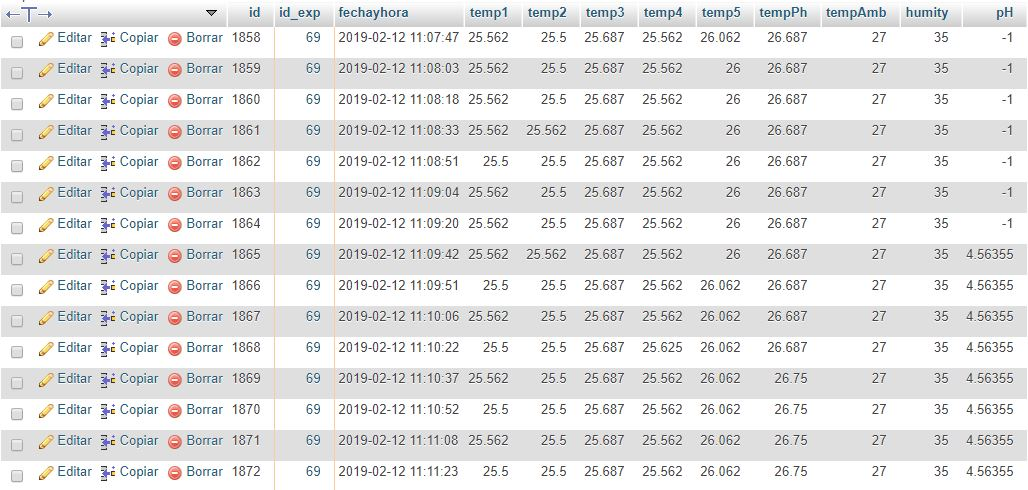
\includegraphics[scale=0.5]{Pruebas/Inserciones.jpg}
    \caption{Captura de mediciones realizadas para la prueba de velocidad}
    \label{fig:pruebasdeInsercion}
\end{figure}
\begin{figure}[H]
    \centering
    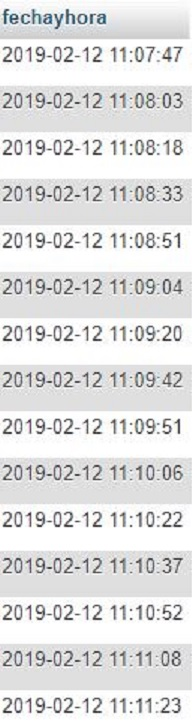
\includegraphics[scale=0.5]{Pruebas/InsercionesZOOM.jpg}
    \caption{Acercamiento de ``fechayhora'' de la tabla de mediciones de pruebas de velocidad}
    \label{fig:pruebasdeInsercionFechayHora}
\end{figure}
\par
Luego, mediante la herramienta \textit{Postman}, fueron realizados tres experimentos. Estos consisten en realizar la consulta de obtención de mediciones a la REST API. En la Figura \ref{fig:pruebasdeConsulta} se presentan los resultados, donde puede evidenciarse una demora con duraciones entre 15 ms y 94 ms para obtener la respuesta. A partir de este rango de tiempo para la respuesta, se asume a la obtención de datos de la \textit{REST API} como excelente para su propósito.
\begin{figure}[h]
    \centering
    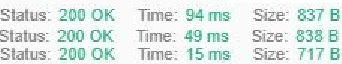
\includegraphics[scale=1]{Pruebas/postman3en1b.jpg}
    \caption{Captura de consulta de mediciones para la prueba de velocidad}
    \label{fig:pruebasdeConsulta}
\end{figure}

\par
Concretadas estas pruebas, se evidenció que el valor mínimo posible para el intervalo de medición de temperatura es de 22 segundos. Ya que el valor de medición de temperatura mínimo definido para el sistema es de 60 segundos, se asumen satisfactorios los resultados, cumpliendo de esta manera el requerimiento no funcional que motivó la misma.

\subsection{Pruebas de campo}
\par En este apartado se exponen un conjunto de pruebas experimentales realizadas con el fin de demostrar que los resultados obtenidos por el sistema en el análisis y optimización de insumos cumplen los requerimientos. 

    \subsubsection{Metodología de pruebas}
        % ---- TERMO -----
        \par Con la finalidad de ejecutar las pruebas se utilizó como macerador un termo\footnote{Termo, adaptación doméstica de un frasco de Dewar} de forma cilíndrica con capacidad volumétrica de 2,5 litros. Al mismo se le realizaron orificios pasantes de forma de incorporar en su interior los sensores de temperatura sumergibles, (Figura \ref{fig:ConstrucMacerador}).
        
        \par En cuanto a la cantidad y ubicación de los sensores dentro del tanque de macerado, considerando el requerimiento RNF006, se buscó la mínima configuración que permitiese realizar mediciones que cubran el radio y la altura del mismo. Para este diseño se utilizó el análisis presentado en el apartado \ref{colocacionDeSensores}. Se tomó como punto de partida la utilización de los vértices de un polígono de tres lados circunscrito en un círculo (vista superior del tanque de maceración, Figura \ref{fig:SensoresEnTanque}, vértices \textbf{A}, \textbf{B} y \textbf{C}). De forma de obtener temperaturas representativas de las distintas profundidades del tanque, se ubicó cada sensor en un vértice desplazado en altura, manteniendo los mismos a distancias verticales equidistantes. De forma adicional, se incorporó un cuarto sensor, centro \textbf{O} del polígono, ubicado en el centroide del tanque. Véase el resultado de la distribución de los sensores \textbf{A'}, \textbf{B'}, \textbf{C'} y \textbf{O'} en la Figura \ref{fig:SensoresEnTanque}.

        \begin{figure}[h]
            \centering
            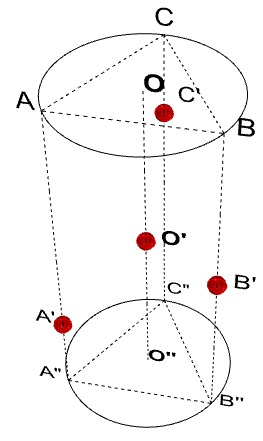
\includegraphics[scale=0.5]{Pruebas/UbicacionSensoresEnTanque-04.jpeg}
            \caption{Esquema representativo de la ubicación de los sensores en el tanque de maceración de forma cilíndrica. La distribución de los sensores A', B', C' y O' (color rojo) yacen en tres niveles de altura distintos, dividiendo el volumen en cuatro secciones verticales de igual tamaño. Para este caso, la altura de los sensores B' y O' se corresponde con el segundo nivel de altura. En vista en planta, los sensores A', B' y C' coinciden con los vértices de un triángulo equilátero (A, B y C) y el sensor O' con el centro de esta figura (O) que se encuentra circunscrita en el cilindro.}
            \label{fig:SensoresEnTanque}
        \end{figure}
        
        \par Los sensores introducidos fueron fijados por medio de pegamento de base siliconada en las posiciones antes indicadas (Figura \ref{fig:ConstrucMacerador}). Para separar los sensores de los bordes del macerador, se utilizaron piezas de poliestireno expandido fijadas entremedio de cada sensor de temperatura y el borde interno del termo.
        Con la finalidad de disminuir la pérdida de calor producida por las perforaciones realizadas para introducir estos sensores, se procedió a aplicar sellador siliconado  en los orificios.
        
        \par Se despreció la posible toxicidad del contacto entre el líquido y el pegamento siliconado. Esta decisión esta basada en que el preparado será utilizado para la realización de las pruebas, y desechado al final de cada una no siendo destinado  al consumo.
        
        \par El termo utilizado cuenta con pico vertedor. El mismo facilita la extracción de muestras sin la necesidad de exponer toda la templa a la temperatura ambiente que produciría la disminución de temperatura y, por tanto, la alteración del experimento.
        
        \par Durante la construcción del macerador, se identificó que el mismo perdía temperatura a un ritmo mayor al aceptable. Por tanto, se procedió a colocar el macerador dentro de un bolso térmico de manera de aumentar el aislamiento. (Figura \ref{fig:ConstrucAislamTerm}).
        
        % ------- pH --------
        \par El sensor de pH fue calibrado para cada una de las maceraciones de prueba realizadas, requerimiento para mejorar la precisión de las mediciones obtenidas señalado en la subsección \ref{subseccionConsideracionesPreviasSensores}.
        
        \par La calibración del sensor de pH consiste en la aplicación de una secuencia de pasos, en los que se ajusta un parámetro mediante software, durante una medición de pH de una solución con un valor estable conocido con el objetivo de mejorar el resultado obtenido. Para este procedimiento, son utilizadas dos soluciones \textbf{buffers} \footnote{Solución química que posee un valor de pH conocido.} cuyos valores (mínimo y máximo) encierran al rango de valores a ser medidos en el experimento. En este caso, el rango de medición varía entre 5 y 6, por tanto, se utilizaron soluciones con valores de pH de 4 y 10, véase Figura \ref{fig:CalibrPhimetro} del Anexo. Luego, esta secuencia inicia con la inmersión de la sonda dentro de la solución \textbf{buffer}. A continuación, se realiza una medición, y se ajusta el resultado mediante un parámetro para este fin. Finalmente, se repite este procedimiento entre las dos soluciones hasta arribar a un valor de ajuste que permita obtener un resultado lo más preciso posible para ambas.
        
        \par Las mediciones de pH se realizaron a partir de una muestra alojada en un recipiente de aluminio refrigerado (figura \ref{fig:MedicPH}) para disminuir la temperatura de la solución a la temperatura de calibración (ver Tabla \ref{tablePhvsTemp}). De forma adicional, dentro del recipiente se alojó un sensor de temperatura con el fin de indicar la temperatura de la templa al momento de la medición de pH.
        
        % ------ Temperatura ------
        \par Al comienzo de un experimento de macerado debe realizarse una infusión entre agua y malta. Ambas en cantidades que deben ser medidas, y en el caso del agua hallarse a una temperatura inicial. Con el fin de medir la cantidad de malta se utilizó una balanza y un recipiente destinado a contenerla. Luego, para calentar y fraccionar el agua utilizada en las pruebas, se empleó una olla de acero inoxidable de cinco litros y un recipiente medidor de un litro. La cantidad y temperatura del agua utilizada en cada uno de los experimentos fue acorde a las indicaciones provistas por la aplicación, pantalla de detalle de maceración, (mencionado en la subsección \ref{DescripPantallaDetalleMaceración}).
        
        \par En cuanto a la identificación de la temperatura inicial del agua, se utilizó una funcionalidad provista por el sistema. En forma conjunta, esta funcionalidad consiste de un sensor de temperatura destinado a este fin y la utilización de la función para la realización de mediciones ``informar valores actuales'', la cual puede encontrarse en la pantalla principal de la aplicación.
        
        \par En particular, para las pruebas con maceraciones escalonadas, para que un cierto volumen de maceración aumente su temperatura a un valor objetivo (escalón de temperatura) debe ser agregada agua a temperatura de hervor. La cantidad de agua caliente que debe ser incorporada al mosto para producir un salto de temperatura es provista por la aplicación en la pantalla ``detalle de maceración'' (mencionado en la subsección \ref{DescripPantallaDetalleMaceración}).
        
        % ------ Densidad ----
        \par Al final de cada experimento de maceración debe ingresarse, en la aplicación, el valor correspondiente a la densidad final obtenida del proceso. La medición de la misma fue realizada mediante la utilización de un densímetro, de escala 1 - 1,1 [$kg/m^3$], y una probeta, de 170 [$cm^3$]. El procedimiento consiste en la toma de una muestra del mosto que es incorporada dentro de la probeta, finalmente, se introduce el densímetro en la probeta para realizar la medición correspondiente.
        
        % ------ Mediciones ----
        \par Para la realización de los experimentos se optó por utilizar intervalos de medición de 1 minuto para la medición de temperatura y 10 minutos para la obtención de la medida de pH. Si bien el sistema soporta mayor frecuencia de medición de pH, la limitante del volumen del recipiente empleado no permite obtener una cantidad de templa de la cual se puedan extraer demasiadas muestras sin que el total de estas extracciones afecte al resultado final. La cantidad de pruebas se definieron acorde a la realización de diez experimentos por cada tipo de maceración planteada. Es a partir de tres experimentos, que el sistema comienza a realizar ajustes sobre el cálculo de insumos. Luego, con diez experimentos es posible observar el ajuste de este valor.
        
        % ---- Grano ----
        \par La malta utilizada para todos los experimentos proviene del mismo lote, y es resguardada en las mismas condiciones. De esta manera puede asegurarse que cualquier cambio de rendimiento obtenido se debe únicamente a la cantidad de insumo utilizado. Definiendo así, las mismas condiciones para todos los experimentos.
        
        En el Anexo \ref{AnexoFotografias} se ubican una serie de imágenes relacionadas a la construcción del sistema y a los procedimientos involucrados en el proceso de maceración.
        
        \subsubsection{Recetas y tipos de maceración utilizadas}
        
        \par Para llevar a cabo los experimentos se planificaron las siguientes maceraciones:
        \hfill \break
        \hfill \break
        \begin{longtable}{p{0.6cm} p{0.6cm} p{12.8cm}}

        \endfirsthead
 
        \endhead
 
        \endfoot
 
        \endlastfoot


        \multicolumn{3}{l}{\textbf{Pilsen Lager - Simple}}\\
        & & \\
        & \multicolumn{2}{l}{Tipo de Maceración: Simple} \\
        & \multicolumn{2}{l}{Volumen: 2 litros}  \\
        & \multicolumn{2}{l}{Densidad específica deseada: 1.070} \\
        & & \\
        & \multicolumn{2}{l}{Granos:} \\
        & & Nombre: Pilsener \\
        & & Porcentaje de utilización: 100\% \\
        & & Extracto Potencial: 80\% \\
        & & \\
        & \multicolumn{2}{l}{Intervalos:} \\
        & & Duración: 60 minutos \\
        & & Temperatura objetivo: 65°C \\
        & & Desvío de temperatura tolerado: ±3°C \\
        & & pH: 5.4 \\
        & & Desvío de pH tolerado: ±0.2 \\
        & & \\
        & & \\
        \multicolumn{3}{l}{\textbf{Pilsen Lager - Escalonada}}\\
        & & \\
        
        & \multicolumn{2}{l}{Tipo de Maceración: Escalonada} \\
        & \multicolumn{2}{l}{Volumen: 2 litros}  \\
        & \multicolumn{2}{l}{Densidad específica deseada: 1.070} \\
        & & \\
        & \multicolumn{2}{l}{Granos:} \\
        & & Nombre: Pilsener \\
        & & Porcentaje de utilización: 100\% \\
        & & Extracto Potencial: 80\% \\
        & & \\
        & \multicolumn{2}{l}{Intervalos:} \\
        & & Duración: 20 minutos \\
        & & Temperatura objetivo: 45°C \\
        & & Desvío de temperatura tolerado: ±3°C \\
        & & pH: 5.4 \\
        & & Desvío de pH tolerado: ±0.2 \\
        & & \\
        & & Duración: 20 minutos \\
        & & Temperatura objetivo: 55°C \\
        & & Desvío de temperatura tolerado: ±3°C \\
        & & pH: 5.4 \\
        & & Desvío de pH tolerado: ±0.2 \\
        & & \\
        & & Duración: 20 minutos \\
        & & Temperatura objetivo: 65°C \\
        & & Desvío de temperatura tolerado: ±3°C \\
        & & pH: 5.4 \\
        & & Desvío de pH tolerado: ±0.2 \\

        \end{longtable}
    
    \subsubsection{Valores calculados para cada receta}
    %\hfill \break
    \par A continuación se visualizan los valores calculados por la aplicación para conocer la cantidad de insumos necesaria para realizar la maceración según la planificación correspondiente.
    %\par La cantidad de insumos ajustados se empieza a visualizar a partir de la tercer fila, acorde a la regla de negocio planteada en el capítulo de \ref{}.
    \par Leyenda de las Tablas \ref{tab:ResultadosPilsenSimple} y \ref{tab:ResultadosPilsenEscalonada}: R.U. = rendimiento utilizado, I.U. = cantidad de insumos Utilizado, D.O. = Densidad Obtenida, R.O. = rendimiento obtenido, R.O. = rendimiento promedio y A.I. = ajuste de insumos.
    
        \subsubsection{Pilsen Lager - Simple}
        
        \begin{longtable}{|p{1cm}|p{1.7cm}|p{2cm}|p{2cm}|p{2cm}| p{1cm}| p{1cm}|}
        \hline
        Exp. %Experimento
        & \multicolumn{1}{c|}{R.U.} %Rendimiento utilizado%
        & \multicolumn{1}{c|}{I.U.} %Insumos utilizados%
        & \multicolumn{1}{c|}{D.O.} %Densidad Obtenida
        & \multicolumn{1}{c|}{R.O.} %Rendimiento obtenido
        & \multicolumn{1}{c|}{R.P.} %Rendimiento promedio
        & \multicolumn{1}{c|}{A.I.} %Insumos ajustados
        \\
        \endfirsthead
        
        \endhead
 
        \endfoot
        
        \hline
        \caption{Tabla de resultados Pilsen Lager simple\label{tab:ResultadosPilsenSimple}}\\
        \endlastfoot
        \hline
            %1er experimento
             \multicolumn{1}{|c|}{1} 
             & \multicolumn{1}{c|}{70\%} %RU
             & \multicolumn{1}{c|}{0.36 Kg.} %IU
             & \multicolumn{1}{c|}{1.06 } %DO
             & \multicolumn{1}{c|}{60.13\%} %RO
             & \multicolumn{1}{c|}{60.13\%} %RP
             & \multicolumn{1}{c|}{-} %AI
             \\
             \hline
             
             %2do experimento
             \multicolumn{1}{|c|}{2} 
             & \multicolumn{1}{c|}{70\%} %RU
             & \multicolumn{1}{c|}{0.36 Kg.} %IU
             & \multicolumn{1}{c|}{1.062} %DO
             & \multicolumn{1}{c|}{62.2\%} %RO
             &\multicolumn{1}{c|}{61.165\%} %RP
             &\multicolumn{1}{c|}{-} %AI
             
             \\
             \hline
             
             %3er experimento
             \multicolumn{1}{|c|}{3} 
             & \multicolumn{1}{c|}{70\%} %RU
             & \multicolumn{1}{c|}{0.36 Kg.} %IU
             & \multicolumn{1}{c|}{1.065} %DO
             & \multicolumn{1}{c|}{62.53\%} %RO
             &\multicolumn{1}{c|}{62.54\%} %RP 
             &\multicolumn{1}{c|}{0.37356 Kg.} %AI
             
             \\
             \hline
             
             %4to experimento
             \multicolumn{1}{|c|}{4} 
             & \multicolumn{1}{c|}{62.54\%}  %RU
             & \multicolumn{1}{c|}{0.37356 Kg.} %IU
             & \multicolumn{1}{c|}{1.067} %DO
             & \multicolumn{1}{c|}{67.37\%} %RO
             & \multicolumn{1}{c|}{63.75\%} %RP
             & \multicolumn{1}{c|}{0.37777 Kg.} %AI
             
             \\
             \hline
             
             %5to experimento
             \multicolumn{1}{|c|}{5} 
             & \multicolumn{1}{c|}{63.75\%} 
             & \multicolumn{1}{c|}{0.37777 Kg.}
             & \multicolumn{1}{c|}{1.069}
             & \multicolumn{1}{c|}{69.45\%}
             & \multicolumn{1}{c|}{64.89\%} 
             & \multicolumn{1}{c|}{0.38221 Kg.} 

             \\
             \hline
             
             %6to experimento
             \multicolumn{1}{|c|}{6} 
             & \multicolumn{1}{c|}{64.89\%}  
             & \multicolumn{1}{c|}{0.38221 Kg.} 
             & \multicolumn{1}{c|}{1.072}
             & \multicolumn{1}{c|}{72.57\%}
             & \multicolumn{1}{c|}{66.17\%} 
             &\multicolumn{1}{c|}{0.39111 Kg.} 

             \\
             \hline
             
             %7mo experimento
             \multicolumn{1}{|c|}{7} 
             & \multicolumn{1}{c|}{66.17\%}  
             & \multicolumn{1}{c|}{0.39111 Kg.} 
             & \multicolumn{1}{c|}{1.07}
             & \multicolumn{1}{c|}{70.49\%}
             & \multicolumn{1}{c|}{66.78\%} 
             & \multicolumn{1}{c|}{0.37673 Kg.} 
             \\
             \hline
             
             %8vo experimento
             \multicolumn{1}{|c|}{8} 
             & \multicolumn{1}{c|}{66.78\%}  
             & \multicolumn{1}{c|}{0.37673 Kg.}
             & \multicolumn{1}{c|}{1.068}
             & \multicolumn{1}{c|}{68.41\%}
             & \multicolumn{1}{c|}{66.99\%} 
             & \multicolumn{1}{c|}{0.36486 Kg.} 
             
             \\
             \hline
             
             %9no experimento
             \multicolumn{1}{|c|}{9} 
             & \multicolumn{1}{c|}{66.99\%}  
             & \multicolumn{1}{c|}{0.36486 Kg.} 
             & \multicolumn{1}{c|}{1.068}
             & \multicolumn{1}{c|}{68.41\%}
             & \multicolumn{1}{c|}{67.14\%} 
             & \multicolumn{1}{c|}{0.36401 Kg.} 
             \\
             \hline
             
             %10mo experimento
             \multicolumn{1}{|c|}{10} 
             & \multicolumn{1}{c|}{67.14\%} 
             & \multicolumn{1}{c|}{0.36401 Kg.} 
             & \multicolumn{1}{c|}{1.07}
             & \multicolumn{1}{c|}{70.49\%}
             & \multicolumn{1}{c|}{67.48\%} 
             & \multicolumn{1}{c|}{0.37286 Kg.} 
             
             \\
             \hline
        
        \end{longtable}
        
    
 \subsubsection{Pilsen Lager - Escalonada}

\begin{longtable}{|p{1cm}|p{1.7cm}|p{2cm}|p{2cm}|p{2cm}| p{1cm}| p{1cm}|}
        \hline
        Exp. %Experimento
        & \multicolumn{1}{c|}{R.U.} %Rendimiento utilizado%
        & \multicolumn{1}{c|}{I.U.} %Insumos utilizados%
        & \multicolumn{1}{c|}{D.O.} %Densidad Obtenida
        & \multicolumn{1}{c|}{R.O.} %Rendimiento obtenido
        & \multicolumn{1}{c|}{R.P.} %Rendimiento promedio
        & \multicolumn{1}{c|}{A.I.} %Insumos ajustados
        \\
        \endfirsthead
        
        \endhead
 
        \endfoot
        
        \hline
        
        \caption{Tabla de resultados Pilsen Lager escalonada\label{tab:ResultadosPilsenEscalonada}}\\
        \endlastfoot
        
        \hline
             \multicolumn{1}{|c|}{1} 
             & \multicolumn{1}{c|}{70\%} 
             & \multicolumn{1}{c|}{0.36 Kg.}
             & \multicolumn{1}{c|}{1.052}
             & \multicolumn{1}{c|}{51.92\%}
             & \multicolumn{1}{c|}{51.92\%} 
             & \multicolumn{1}{c|}{-} \\
             \hline
             
             \multicolumn{1}{|c|}{2} 
             & \multicolumn{1}{c|}{70\%}  
             & \multicolumn{1}{c|}{0.36 Kg.}
             & \multicolumn{1}{c|}{1.062}
             & \multicolumn{1}{c|}{62.2\%}
             & \multicolumn{1}{c|}{57.06\%} 
             & \multicolumn{1}{c|}{-} \\
             \hline
             
             \multicolumn{1}{|c|}{3} 
             & \multicolumn{1}{c|}{70\%} 
             & \multicolumn{1}{c|}{0.36 Kg.}
             & \multicolumn{1}{c|}{1.065}
             & \multicolumn{1}{c|}{65.3\%}
             & \multicolumn{1}{c|}{59.8\%}
             & \multicolumn{1}{c|}{0.37356 Kg.} \\
             \hline
             
             \multicolumn{1}{|c|}{4} 
             & \multicolumn{1}{c|}{59.8\%}  
             & \multicolumn{1}{c|}{0.37356 Kg.}
             & \multicolumn{1}{c|}{1.064}
             & \multicolumn{1}{c|}{64.27\%}
             & \multicolumn{1}{c|}{60.92\%}
             & \multicolumn{1}{c|}{0.36529 Kg.} \\
             \hline
             
             \multicolumn{1}{|c|}{5} 
             & \multicolumn{1}{c|}{60.92\%}  
             & \multicolumn{1}{c|}{0.36529 Kg.} 
             & \multicolumn{1}{c|}{1.065}
             & \multicolumn{1}{c|}{65.3\%} 
             & \multicolumn{1}{c|}{61.79\%}             
             & \multicolumn{1}{c|}{0.36828 Kg.} \\
             \hline
             
             \multicolumn{1}{|c|}{6} 
             & \multicolumn{1}{c|}{61.79\%}  
             & \multicolumn{1}{c|}{0.36828 Kg.} 
             & \multicolumn{1}{c|}{1.074}
             & \multicolumn{1}{c|}{74.66\%} 
             & \multicolumn{1}{c|}{63.94\%}             
             & \multicolumn{1}{c|}{0.40727 Kg.} \\
             \hline
             
             \multicolumn{1}{|c|}{7} 
             & \multicolumn{1}{c|}{63.94\%}  
             & \multicolumn{1}{c|}{0.40727 Kg.} 
             & \multicolumn{1}{c|}{1.07}
             & \multicolumn{1}{c|}{70.49\%} 
             & \multicolumn{1}{c|}{64.87\%}
             & \multicolumn{1}{c|}{0.38094 Kg.} \\
             \hline
             
             \multicolumn{1}{|c|}{8} 
             & \multicolumn{1}{c|}{64.87\%}  
             & \multicolumn{1}{c|}{0.38094 Kg.} 
             & \multicolumn{1}{c|}{1.072}
             & \multicolumn{1}{c|}{72.57\%}
             & \multicolumn{1}{c|}{65.89\%}
             & \multicolumn{1}{c|}{0.38705 Kg.} \\
             \hline
             
             \multicolumn{1}{|c|}{9} 
             & \multicolumn{1}{c|}{66.86\%}  
             & \multicolumn{1}{c|}{0.38705 Kg.} 
             & \multicolumn{1}{c|}{1.068}
             & \multicolumn{1}{c|}{68.41\%}
             & \multicolumn{1}{c|}{66.12\%}
             & \multicolumn{1}{c|}{0.36461 Kg.} \\
             \hline
             
             \multicolumn{1}{|c|}{10} 
             & \multicolumn{1}{c|}{66.12\%} 
             & \multicolumn{1}{c|}{0.36461 Kg.} 
             & \multicolumn{1}{c|}{1.07}
             & \multicolumn{1}{c|}{70.49\%}
             & \multicolumn{1}{c|}{66.56\%}
             & \multicolumn{1}{c|}{0.37341 Kg.} \\
             \hline
        
    \end{longtable}
    
    %\subsubsection{Resultados obtenidos}
        \par Para cada receta realizada se muestran las gráficas de promedio de temperatura y pH obtenidas por la aplicación. Las mismas se presentan en el Anexo \ref{GraficasPruebasCampo}.
    
    \subsubsection{Evaluación}
        \par En las pruebas de campo se evidenció que el ajuste de la cantidad de insumos realizada por el sistema produce resultados correctos, esto es, cuando el valor de rendimiento es menor al deseado incrementa la cantidad de granos de manera de compensar este sub-rendimiendo, y lo mismo ocurre en caso contrario con un sobre-rendimiento. Esta compensación representa el objetivo de esta funcionalidad, la cual es asistir al productor a partir de una herramienta de optimización de insumos en función de un ajuste utilizando el rendimiento del equipo.
        
        \par Cabe señalar que si bien pueden parecer reducidos los cambios en los valores de insumos, los mismos corresponden a un preparado de un volumen reducido. Estos cambios crecerán en forma proporcional al tamaño del preparado, constituyéndose en valores más significativos conforme a este incremento, dado que, los cálculos realizados son linealmente proporcionales al volumen de producción.
        
        \par Por tanto, puede concluirse que esta funcionalidad del sistema se comporta de la manera esperada, y por tanto, correcta. 